\documentclass[11pt,a4paper]{article}

\usepackage{iftex}
\ifXeTeX
  \usepackage{fontspec}
\else
  \usepackage[T1]{fontenc}
  \usepackage[utf8]{inputenc}
  \usepackage{lmodern}
\fi
\usepackage[french]{babel}
\usepackage[margin=2.3cm]{geometry}
\usepackage{amsmath,amssymb,amsthm}
\usepackage{graphicx}
\usepackage{booktabs}
\usepackage{tabularx}
\usepackage{float}
\usepackage{caption}
\usepackage{subcaption}
\usepackage{xcolor}
\usepackage{listings}
\usepackage{enumitem}
\usepackage[colorlinks=true,linkcolor=blue!50!black,urlcolor=blue!50!black,citecolor=blue!50!black]{hyperref}

\graphicspath{{../../results/part3/}}
\setlist{itemsep=2pt,topsep=4pt}

\newtheorem{proposition}{Proposition}
\theoremstyle{remark}
\newtheorem*{remarque}{Remarque}

\newcommand{\Deg}{\mathrm{Deg}}
\newcommand{\Att}{\mathrm{Att}}
\newcommand{\HCat}{\mathrm{HCat}}

\lstset{
  language=Python,
  basicstyle=\ttfamily\small,
  keywordstyle=\color{blue!60!black}\bfseries,
  commentstyle=\color{green!40!black}\itshape,
  stringstyle=\color{red!50!black},
  frame=single, rulecolor=\color{gray!50},
  backgroundcolor=\color{gray!5},
  showstringspaces=false, columns=fullflexible,
  breaklines=true, xleftmargin=4pt, xrightmargin=4pt
}

\title{\textbf{Partie 3 --- Visualising Acceptability Degree Spaces}\\[4pt]
\large Sémantique weighted h-categorizer : convergence, enveloppe convexe et cartes de densité}
\author{Mohamed Amine Benhamaid}
\date{\today}

\begin{document}
\maketitle

\begin{abstract}
Nous implémentons la sémantique \emph{weighted h-categorizer} avec un critère d'arrêt
paramétré par $\varepsilon>0$, puis nous étudions l'espace des degrés d'acceptabilité
$S=\HCat([0,1]^{|A|})$ en échantillonnant $100\,000$ vecteurs de poids uniformes pour
17 frameworks de 2 à 6 arguments. Nous montrons que $S$ admet une description exacte,
$\{x\ge 0 : x_a(1+\sum_{b\to a}x_b)\le 1\}$, et que la densité des points échantillonnés
vaut $|\det J_g(x)|$. Cela fournit une vérité terrain pour juger l'enveloppe convexe,
qui surestime $S$ de 7\,\% (2 arguments) à 22\,\% (6 arguments), et les cartes de densité.
Celles-ci sont robustes au ré-échantillonnage, avec une erreur qui décroît en $1/\sqrt N$
(environ 4\,\% en variation totale pour $N=100\,000$).
\end{abstract}

\tableofcontents
\newpage

%======================================================================
\section{Sémantique weighted h-categorizer}
%======================================================================

\subsection{Définition}

Un framework d'argumentation pondéré est un triplet $(A,R,w)$, où $A$ est un ensemble fini
d'arguments, $R\subseteq A\times A$ une relation d'attaque et $w:A\to[0,1]$ un poids initial.
On note $\Att(a)=\{b \mid (b,a)\in R\}$. La sémantique weighted h-categorizer
(Amgoud \emph{et al.}, 2017) associe à chaque argument le degré
\begin{equation}\label{eq:hcat}
  \Deg(a) \;=\; \frac{w(a)}{1+\sum_{b\in\Att(a)}\Deg(b)} ,
\end{equation}
unique solution de ce système, obtenue comme limite de la suite
\begin{equation}\label{eq:iter}
  f^0(a)=w(a), \qquad f^{k+1}(a) = \frac{w(a)}{1+\sum_{b\in\Att(a)} f^k(b)} .
\end{equation}
On arrête l'itération dès que $\max_{a\in A}|f^{k+1}(a)-f^k(a)|<\varepsilon$.

\subsection{Implémentation}

Le code est dans \texttt{src/part3/hcategorizer.py}. La relation $R$ est stockée dans une
matrice $M\in\{0,1\}^{n\times n}$ avec $M_{ba}=1$ si et seulement si $b$ attaque $a$. La somme
des degrés des attaquants de tous les arguments s'écrit alors $xM$. On peut ainsi traiter
\emph{simultanément} $N$ vecteurs de poids, rangés en lignes dans une matrice $W$ :

\begin{lstlisting}
def h_categorizer_batch(af, W, epsilon=1e-8, max_iter=100_000):
    if epsilon <= 0:
        raise ValueError("epsilon must be > 0")
    M, x = af.matrix, W.copy()
    for k in range(1, max_iter + 1):
        x_new = W / (1.0 + x @ M)          # equation (2) for all rows at once
        delta = np.max(np.abs(x_new - x))
        x = x_new
        if delta < epsilon:
            return x
    raise RuntimeError("no convergence")
\end{lstlisting}

La fonction \texttt{h\_categorizer(af, weights, epsilon)} traite un seul vecteur, donné sous
forme de dictionnaire ou de liste. Un framework quelconque $(A,R)$ peut être passé en ligne
de commande sous la forme \texttt{"a,b,c : a>b, b>c"}. Grâce à la vectorisation, le calcul
des $100\,000$ vecteurs prend entre 0,02\,s et 0,4\,s selon le framework.

\subsection{Tests sur de petits frameworks}

Les tests (\texttt{tests/test\_part3\_hcategorizer.py}, 19 tests, tous réussis) comparent
le résultat à une forme close, calculée avec $\varepsilon=10^{-12}$ :

\begin{table}[H]
\centering\small
\begin{tabularx}{\linewidth}{lX}
\toprule
Framework & Forme close vérifiée \\
\midrule
$a$, $b$ sans attaque & $\Deg=w$ \\
$a\to b$ & $\Deg(a)=w_a$, \ $\Deg(b)=w_b/(1+w_a)$ \\
$a\leftrightarrow b$ & $x_a-x_b=w_a-w_b$ et $x_b(1+x_a)=w_b$ ; pour $w\equiv 1$ :
$x=(\sqrt5-1)/2\approx 0{,}618$ \\
$a\to a$ (auto-attaque) & $x=(-1+\sqrt{1+4w})/2$ \\
chaîne $a\to b\to c$, $w\equiv1$ & $(1,\ 1/2,\ 2/3)$ \\
cycle de longueur 3, $w\equiv1$ & $\Deg\equiv\varphi^{-1}=0{,}618$ (nombre d'or) \\
étoile $a,b\to c$ & $\Deg(c)=w_c/(1+w_a+w_b)$ \\
20 graphes aléatoires (6 arg.) & le résultat est un point fixe de \eqref{eq:hcat} et $0\le\Deg\le w$ \\
divers & $w(a)=0\Rightarrow\Deg(a)=0$ ; version batch $=$ version unitaire ;
$\varepsilon\le 0$ et poids hors de $[0,1]$ rejetés \\
\bottomrule
\end{tabularx}
\caption{Tests de la sémantique sur des frameworks dont les degrés sont connus.}
\end{table}

\subsection{Convergence et rôle de \texorpdfstring{$\varepsilon$}{epsilon}}

\begin{figure}[H]
\centering
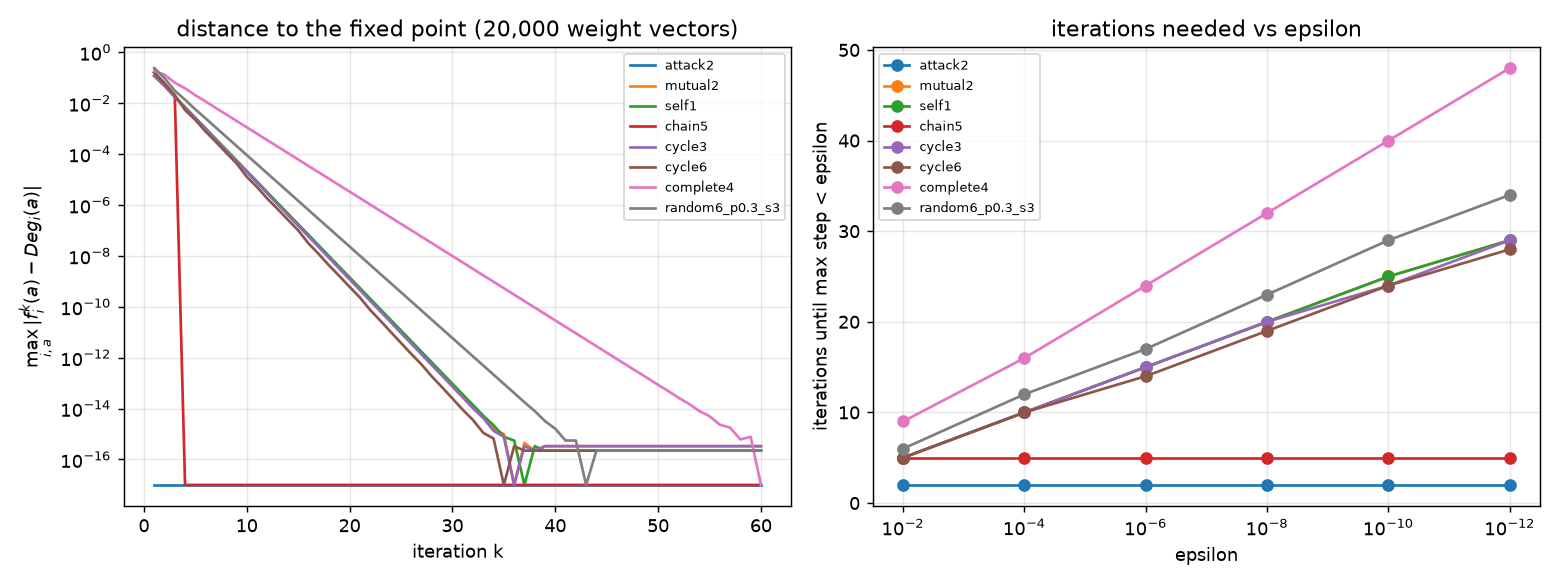
\includegraphics[width=\linewidth]{convergence.png}
\caption{À gauche : distance au point fixe en fonction de l'itération, pour 20\,000 vecteurs
de poids traités ensemble (échelle logarithmique). À droite : nombre d'itérations nécessaires
en fonction de $\varepsilon$.}
\label{fig:conv}
\end{figure}

\begin{table}[H]
\centering\small
\begin{tabular}{lcccccc}
\toprule
$\varepsilon$ & $10^{-2}$ & $10^{-4}$ & $10^{-6}$ & $10^{-8}$ & $10^{-10}$ & $10^{-12}$ \\
\midrule
$a\to b$ / chaîne à 5 (acycliques) & 2 / 5 & 2 / 5 & 2 / 5 & 2 / 5 & 2 / 5 & 2 / 5 \\
$a\leftrightarrow b$, cycle à 3 & 5 & 10 & 15 & 20 & 24--25 & 29 \\
cycle à 6 & 5 & 10 & 14 & 19 & 24 & 28 \\
aléatoire (6 arg., 10 att.) & 6 & 12 & 17 & 23 & 29 & 34 \\
complet à 4 & 9 & 16 & 24 & 32 & 40 & 48 \\
\bottomrule
\end{tabular}
\caption{Nombre d'itérations jusqu'à ce que le pas maximal soit inférieur à $\varepsilon$.}
\end{table}

\begin{enumerate}
\item \textbf{Graphes acycliques : convergence exacte en un nombre fini d'étapes.}
Il faut $(\text{profondeur}+1)$ itérations, car $f^k(a)$ est définitif dès que tous les
ancêtres de $a$ le sont. L'erreur tombe alors à $0$ en flottant, quel que soit $\varepsilon$.
\item \textbf{Graphes cycliques : convergence géométrique.} En échelle logarithmique l'erreur
est une droite. Pour les cycles, on gagne deux décimales toutes les 5 itérations, soit un taux
d'environ $0{,}4\approx\varphi^{-2}=0{,}382$. C'est la valeur absolue de la dérivée de
$x\mapsto 1/(1+x)$ au point fixe $\varphi^{-1}$, atteinte pour des poids égaux à 1 (le pire cas).
Plus il y a d'attaquants, plus la contraction est lente (environ $0{,}56$ pour le graphe
complet à 4 arguments).
\item \textbf{$\varepsilon$ contrôle la précision.} Comparée à une référence calculée avec
$\varepsilon=10^{-15}$, l'erreur finale est toujours inférieure à $\varepsilon$
(entre $0{,}2\,\varepsilon$ et $0{,}3\,\varepsilon$), pour un coût logarithmique en
$1/\varepsilon$. Nous prenons $\varepsilon=10^{-10}$ dans la suite.
\end{enumerate}

%======================================================================
\section{Espace des degrés d'acceptabilité}
%======================================================================

\subsection{Protocole expérimental}

Pour un framework $(A,R)$ donné :
\begin{enumerate}
\item tirer $N=100\,000$ vecteurs $w_i\sim\mathcal U([0,1]^{|A|})$, avec une graine fixée ;
\item calculer $x_i=\HCat(w_i)$ ;
\item construire l'enveloppe convexe des $x_i$ avec Qhull (\texttt{scipy.spatial.ConvexHull}),
en dimension pleine jusqu'à $|A|=6$ ;
\item construire des cartes de densité (heat-maps) : histogrammes 2D de $40\times40$ cases,
en densité par unité de surface. En dimension 3, on ajoute un nuage de points coloré par la
densité et l'enveloppe 3D. Pour $|A|\ge4$, on trace la matrice des projections 2D, où la
projection de l'enveloppe $n$-D est l'enveloppe 2D des points projetés ;
\item tester la résilience : 10 ré-échantillonnages indépendants, comparés par distance
en variation totale (TV), distance de Jensen--Shannon, recouvrement des zones de forte
densité et variabilité du volume de l'enveloppe ;
\item faire varier la structure (sans attaque, attaque simple, attaque mutuelle, auto-attaque,
chaîne, cycle, étoile, graphe complet, graphes aléatoires) et le nombre d'arguments (2 à 6).
\end{enumerate}

\subsection{Description exacte de l'espace \texorpdfstring{$S$}{S}}

L'équation \eqref{eq:hcat} se réécrit $w_a = x_a\bigl(1+\sum_{b\to a}x_b\bigr)$.
L'application $w\mapsto x$ s'inverse donc \emph{explicitement} par $g(x)=x\odot(1+xM)$.

\begin{proposition}\label{prop:S}
Soit $S=\HCat([0,1]^{|A|})$. Alors
\[
S=\Bigl\{x\in\mathbb R^{|A|}_{\ge 0} \;:\; x_a\Bigl(1+\sum_{b\in\Att(a)}x_b\Bigr)\le 1\quad\forall a\in A\Bigr\}.
\]
Si $w\sim\mathcal U([0,1]^{|A|})$, la densité de $x=\HCat(w)$ est
$p(x)=|\det J_g(x)|\,\mathbf 1_S(x)$, avec
$(J_g)_{ac}=\delta_{ac}(1+s_a)+x_aM_{ca}$ et $s=xM$. En particulier
$\mathrm{vol}(S)=\mathbb E_w\bigl[1/|\det J_g(\HCat(w))|\bigr]$.
\end{proposition}

\begin{proof}[Idée de preuve]
Si $x\in S$, alors $g(x)=w\in[0,1]^{|A|}$ et $x$ est un point fixe de \eqref{eq:hcat} pour
ce $w$. Par unicité du point fixe, $x=\HCat(w)$. Inversement, $\HCat(w)\ge0$ et
$g(\HCat(w))=w\le 1$. Comme $g$ est une bijection $C^1$ de $S$ sur $[0,1]^{|A|}$, la formule
du changement de variables donne la densité et le volume.
\end{proof}

La proposition donne une \textbf{vérité terrain} pour juger les deux outils de visualisation.
Les tests vérifient que $g(x_i)=w_i$ à $10^{-10}$ près. Quelques conséquences :
\begin{itemize}
\item $a\to b$ : $S=\{x_b\le 1/(1+x_a)\}$, $p(x)=1+x_a$, $\mathrm{vol}(S)=\ln2=0{,}6931$
(mesuré : $0{,}6936\pm0{,}0004$).
\item La chaîne à 3 et l'étoile à 3 ont exactement le même volume,
$3\ln3-4\ln2=0{,}5232$ (mesuré : $0{,}5235$ pour les deux), alors que leurs formes diffèrent.
\item Pour un graphe acyclique, $J_g$ est triangulaire, donc $p(x)=\prod_a(1+s_a)\ge1$.
On observe aussi $p\ge1$ sur tous nos graphes cycliques.
\end{itemize}

\subsection{Résultats globaux}

\begin{table}[H]
\centering\footnotesize
\setlength{\tabcolsep}{4pt}
\begin{tabular}{lrrrrrrrrrr}
\toprule
Framework & $|A|$ & $|R|$ & iter & vol(hull) & vol($S$) & vide & dens.\ max & TV & Jacc.\ HDR50 & CV vol \\
\midrule
isolated2 & 2 & 0 & 1 & 0.9997 & 1.0000 & 0.0\,\% & 1.00 & 0.071 & (0.29)$^*$ & 0.006\,\% \\
attack2 ($a\to b$) & 2 & 1 & 2 & 0.7473 & 0.6936 & 7.3\,\% & 2.00 & 0.059 & 0.66 & 0.13\,\% \\
mutual2 ($a\leftrightarrow b$) & 2 & 2 & 25 & 0.6162 & 0.5808 & 5.9\,\% & 2.23 & 0.055 & 0.56 & 0.09\,\% \\
attack2\_self & 2 & 2 & 25 & 0.5153 & 0.5057 & 2.0\,\% & 2.82 & 0.051 & 0.63 & 0.05\,\% \\
\midrule
chain3 & 3 & 2 & 3 & 0.5878 & 0.5235 & 11.3\,\% & 3.00 & 0.062 & 0.57 & 0.16\,\% \\
cycle3 & 3 & 3 & 24 & 0.4720 & 0.4083 & 13.7\,\% & 4.40 & 0.058 & 0.64 & 0.23\,\% \\
star3 & 3 & 2 & 2 & 0.5993 & 0.5235 & 12.9\,\% & 3.00 & 0.061 & 0.55 & 0.49\,\% \\
complete3 & 3 & 6 & 34 & 0.3029 & 0.2684 & 11.4\,\% & 6.64 & 0.052 & 0.49 & 0.27\,\% \\
\midrule
chain4 & 4 & 3 & 4 & 0.4498 & 0.3882 & 14.4\,\% & 4.96 & 0.062 & 0.56 & 0.19\,\% \\
cycle4 & 4 & 4 & 24 & 0.3669 & 0.3072 & 17.0\,\% & 6.52 & 0.060 & 0.61 & 0.31\,\% \\
complete4 & 4 & 12 & 40 & 0.1238 & 0.1073 & 14.1\,\% & 22.7 & 0.047 & 0.47 & 0.48\,\% \\
random4 & 4 & 3 & 25 & 0.4514 & 0.4024 & 11.5\,\% & 4.43 & 0.063 & 0.57 & 0.14\,\% \\
\midrule
chain5 & 5 & 4 & 5 & 0.3414 & 0.2890 & 16.9\,\% & 7.72 & 0.063 & 0.55 & 0.24\,\% \\
cycle5 & 5 & 5 & 24 & 0.2761 & 0.2279 & 19.0\,\% & 10.4 & 0.061 & 0.61 & 0.27\,\% \\
random5 & 5 & 8 & 25 & 0.1645 & 0.1372 & 18.4\,\% & 19.7 & 0.056 & 0.59 & 0.76\,\% \\
\midrule
cycle6 & 6 & 6 & 24 & 0.2031 & 0.1697 & 19.7\,\% & 16.4 & 0.062 & 0.60 & 0.35\,\% \\
random6 & 6 & 10 & 29 & 0.1075 & 0.0880 & 21.7\,\% & 41.4 & 0.055 & 0.59 & 0.68\,\% \\
\bottomrule
\end{tabular}
\caption{Résultats pour $N=100\,000$ et 10 ré-échantillonnages. \emph{vide} : part du volume
de l'enveloppe qui n'appartient pas à $S$ (Monte-Carlo, 200\,000 points testés avec la
proposition~\ref{prop:S}). \emph{TV} : distance en variation totale moyenne entre les heat-maps
$40\times40$ de deux ré-échantillonnages. \emph{HDR50} : ensemble minimal de cases contenant
50\,\% de la masse (zone de forte densité). \emph{CV vol} : coefficient de variation du volume
de l'enveloppe. $^*$Pour une densité uniforme, la HDR50 n'est pas définie de façon unique.}
\label{tab:res}
\end{table}

\subsection{Analyse de l'enveloppe convexe}

\begin{figure}[H]
\centering
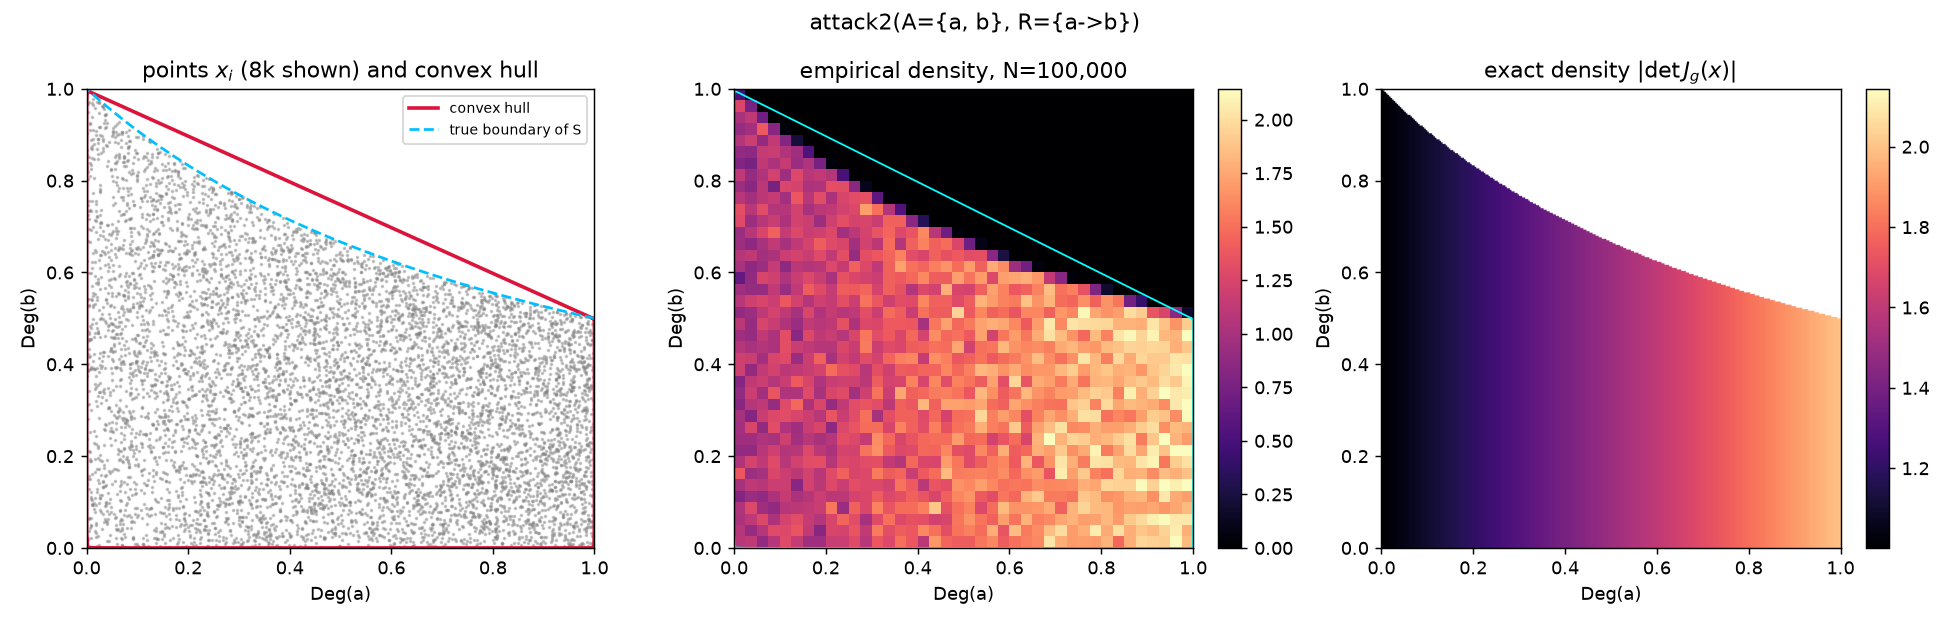
\includegraphics[width=\linewidth]{space_attack2.png}
\caption{$a\to b$. À gauche : points $x_i$, enveloppe convexe (rouge) et vraie frontière de
$S$ (pointillés). Au centre : densité empirique. À droite : densité exacte $1+x_a$.}
\label{fig:attack2}
\end{figure}

\begin{enumerate}
\item \textbf{$S$ n'est pas convexe dès qu'il y a une attaque.} Les contraintes
$x_a+x_ax_b\le1$ sont bilinéaires. Pour $a\to b$, la frontière $x_b=1/(1+x_a)$ est une
fonction convexe, et la région située sous elle n'est pas convexe
(figure~\ref{fig:attack2}). L'enveloppe est alors le trapèze
$(0,0),(1,0),(1,\tfrac12),(0,1)$, d'aire $3/4$, contre $\ln 2$ pour $S$. On a donc
\textbf{7,6\,\% de volume vide} en théorie, 7,3\,\% mesuré. L'enveloppe convexe
\emph{surestime} toujours l'ensemble des degrés atteignables.
\item \textbf{Le volume vide augmente avec la dimension} : 0\,\% sans attaque ($S$ est un cube),
2 à 7\,\% pour $|A|=2$, 11 à 14\,\% pour $|A|=3$, 11 à 17\,\% pour $|A|=4$, 17 à 19\,\% pour $|A|=5$
et 20 à 22\,\% pour $|A|=6$. Chaque argument attaqué ajoute une face creuse. L'auto-attaque seule
donne l'intervalle $[0,\varphi^{-1}]$, qui est convexe, d'où seulement 2\,\% de vide pour
\texttt{attack2\_self}.
\item \textbf{Le volume de $S$ diminue vite avec le nombre d'attaques} : 1 sans attaque,
$0{,}69$ avec une attaque, $0{,}27$ pour le graphe complet à 3, $0{,}11$ pour le complet à 4,
$0{,}09$ pour \texttt{random6}. Les attaques \emph{compriment} l'espace des degrés.
\item \textbf{Le coût explose avec la dimension.} Le nombre de sommets de l'enveloppe passe de
$\sim\!20$ (2D) à $\sim\!120$ (3D), $\sim\!500$ (4D), $\sim\!1\,400$ (5D) et $\sim\!3\,200$ (6D).
Qhull passe de moins de 0,1\,s à environ 8\,s en 6D. Au-delà de 6 arguments, l'enveloppe en
dimension pleine n'est plus praticable, et les projections 2D restent la seule visualisation
exploitable.
\item \textbf{Les sommets de l'enveloppe sont des points rares.} Ce sont des coins du type
« un argument à 1, ses attaquants à 0 », de faible densité. Avec peu d'échantillons, l'enveloppe
empirique est donc plus petite que l'enveloppe de $S$ : à $N=5\,000$, on obtient même
$\mathrm{vol(hull)}<\mathrm{vol}(S)$ en dimensions 5 et 6.
\end{enumerate}

\subsection{Analyse des cartes de densité}

\begin{figure}[H]
\centering
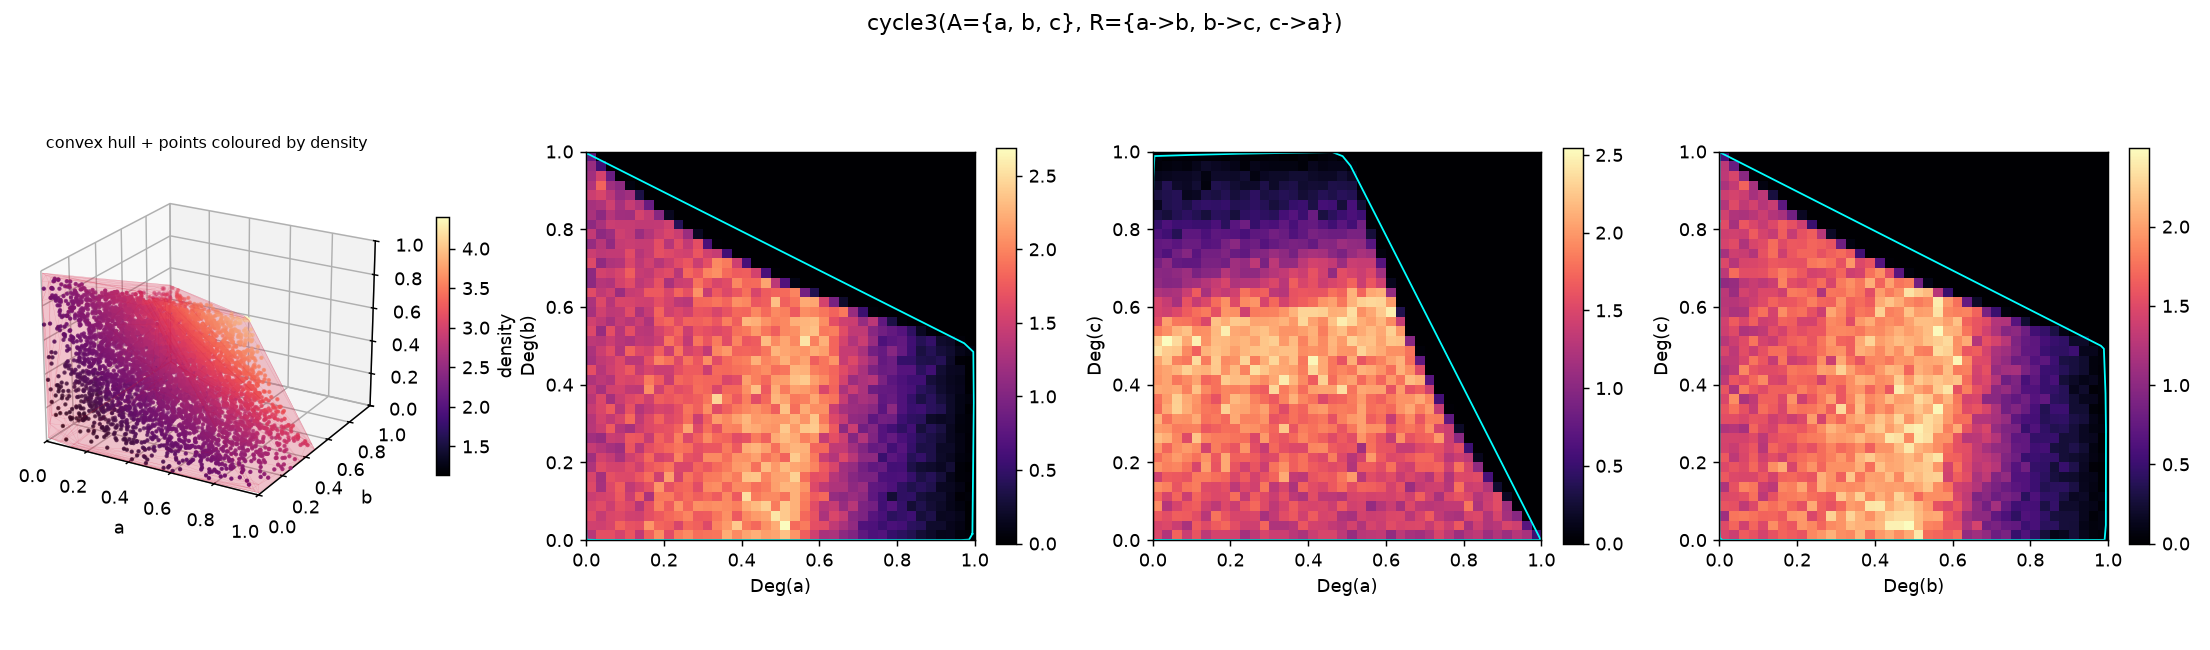
\includegraphics[width=\linewidth]{space_cycle3.png}
\caption{Cycle $a\to b\to c\to a$ : enveloppe 3D et points colorés par la densité exacte
(à gauche), puis densité des trois projections 2D avec l'enveloppe projetée (en cyan).}
\label{fig:cycle3}
\end{figure}

\begin{figure}[H]
\centering
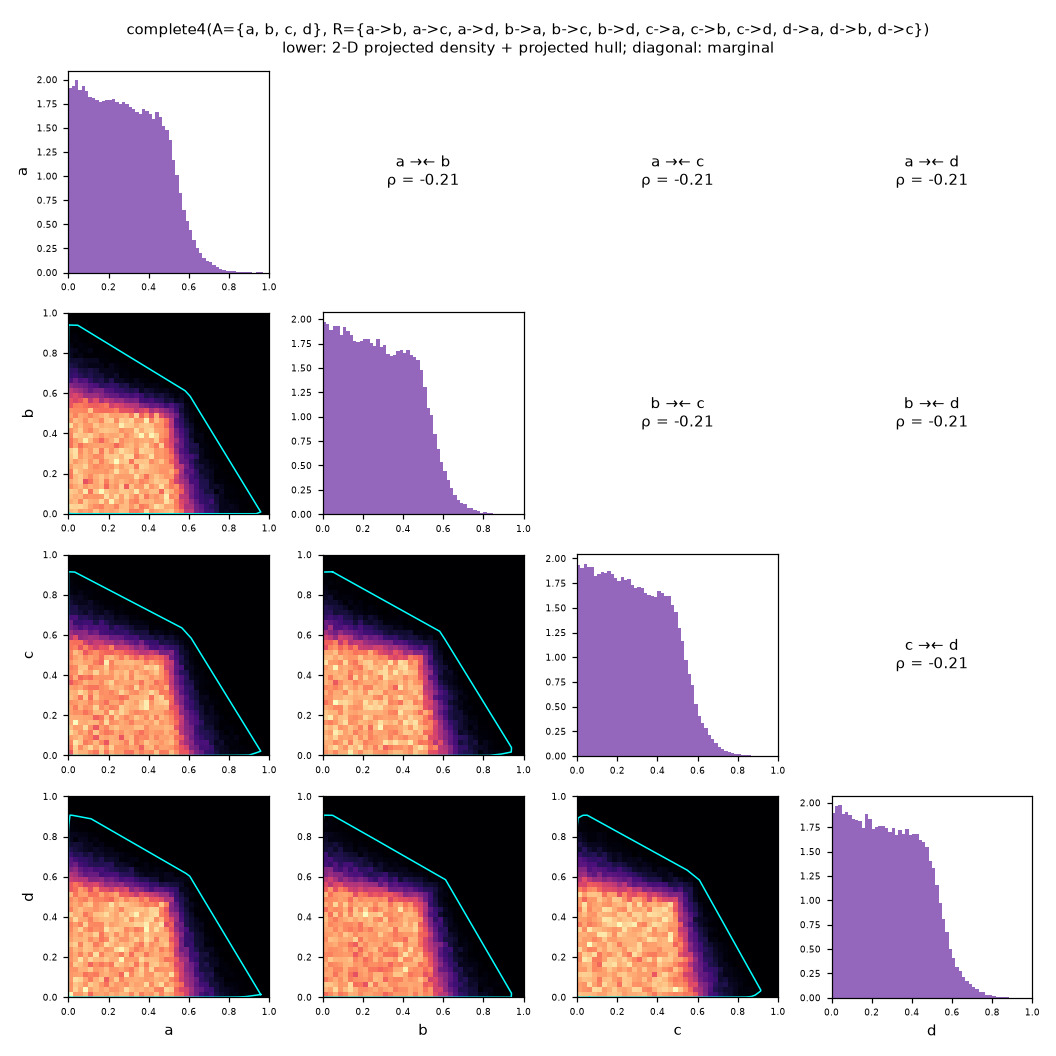
\includegraphics[width=0.78\linewidth]{space_complete4.png}
\caption{Graphe complet à 4 arguments. Sous la diagonale : densités projetées et enveloppe
projetée. Sur la diagonale : distributions marginales. Au-dessus : corrélations.}
\label{fig:complete4}
\end{figure}

\begin{enumerate}
\item \textbf{La densité est forte là où l'attaquant est fort.} Pour $a\to b$, $p=1+x_a$, et la
heat-map empirique reproduit le dégradé exact de 1 à 2 (figure~\ref{fig:attack2}). Quand
$\Deg(a)$ est grand, tous les poids $w_b\in[0,1]$ sont ramenés dans l'intervalle plus court
$[0,1/(1+x_a)]$, d'où une densité plus élevée. Les zones de forte densité sont les régions
comprimées par les attaques. Les zones de faible densité sont celles où un argument attaqué
garde un degré élevé, ce qui impose des attaquants faibles.
\item \textbf{Cycles et graphes complets : un plateau puis une chute brutale.} Pour le cycle à 3
(figure~\ref{fig:cycle3}), la densité est maximale vers $\Deg(a)\approx 0{,}5$--$0{,}6$ et
s'effondre au-delà d'environ $0{,}62$. Pour le graphe complet à 4 (figure~\ref{fig:complete4}),
la masse se concentre dans $[0;0{,}6]^2$ et les marginales sont presque uniformes sur
$[0;0{,}55]$. Les degrés supérieurs à $\varphi^{-1}\approx0{,}62$ demandent des adversaires
faibles : l'enveloppe les englobe, mais ces régions sont presque vides. C'est la différence
entre l'\emph{atteignable} (l'enveloppe) et le \emph{typique} (la heat-map).
\item \textbf{Les degrés moyens suivent la topologie.} Un argument non attaqué a un degré moyen
de $0{,}5$. Un argument attaqué par un argument non attaqué a un degré moyen de
$\tfrac12\ln 2=0{,}347$ (observé : $0{,}3465$). Dans une chaîne, les degrés moyens oscillent
ensuite autour de $0{,}37$--$0{,}38$, et tous les arguments d'un cycle sont vers $0{,}373$.
Dans les graphes complets, la moyenne baisse avec le nombre d'attaquants ($0{,}32$ pour 3
arguments, $0{,}28$ pour 4).
\item \textbf{Les attaques mutuelles créent une corrélation négative} ($\rho=-0{,}21$ entre
chaque paire dans \texttt{complete4}) : un argument fort affaiblit son adversaire.
\item \textbf{La densité maximale augmente fortement avec $|R|$} : 2 pour une attaque, $6{,}6$
pour \texttt{complete3}, $22{,}7$ pour \texttt{complete4}, 41 pour \texttt{random6}. La masse se
concentre dans une partie de plus en plus petite d'un espace lui-même de plus en plus petit.
\end{enumerate}

\subsection{Résilience au ré-échantillonnage}

\begin{figure}[H]
\centering
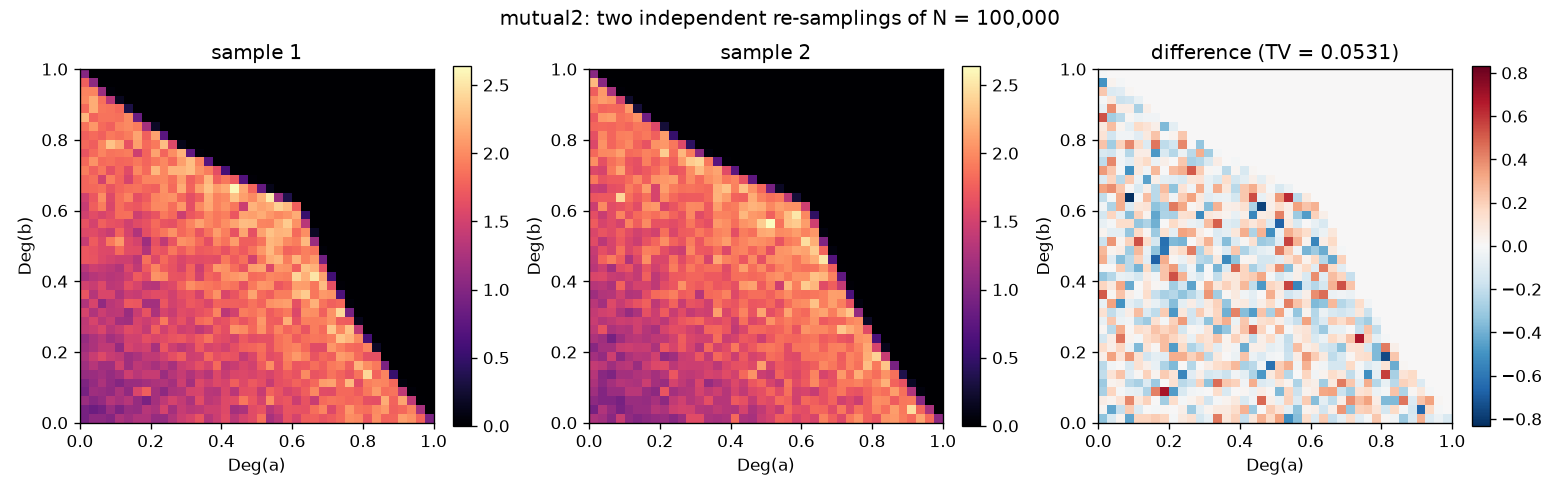
\includegraphics[width=\linewidth]{resampling_mutual2.png}
\caption{$a\leftrightarrow b$ : deux échantillons indépendants de $N=100\,000$ points et leur
différence, qui ne montre que du bruit sans structure spatiale.}
\label{fig:resamp}
\end{figure}

\begin{figure}[H]
\centering
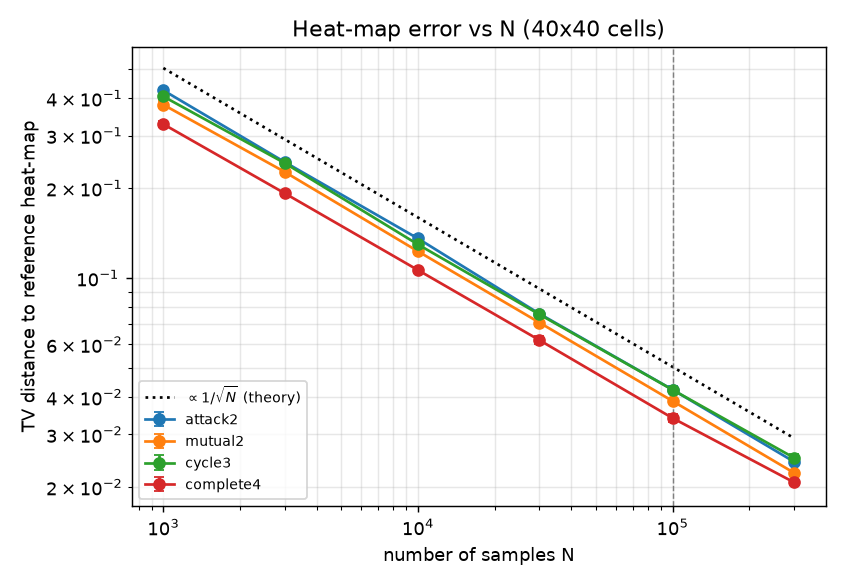
\includegraphics[width=0.62\linewidth]{tv_vs_n.png}
\caption{Distance TV entre la heat-map et une référence, en fonction de $N$. La référence est
la densité exacte intégrée par case pour les frameworks à 2 arguments, et un échantillon de
2 millions de points sinon. La pente vaut $-1/2$.}
\label{fig:tv}
\end{figure}

\begin{enumerate}
\item \textbf{La structure macroscopique est stable.} Deux tirages de 100\,000 points donnent
des heat-maps visuellement identiques, et leur différence n'est que du bruit blanc
(figure~\ref{fig:resamp}). La TV moyenne entre ré-échantillonnages reste entre $0{,}047$ et
$0{,}071$ pour tous les frameworks.
\item \textbf{L'erreur décroît en $1/\sqrt N$.} La TV passe de $\approx0{,}4$ ($N=10^3$) à
$\approx0{,}04$ ($N=10^5$) puis $\approx0{,}024$ ($N=3\cdot10^5$), avec une pente $-1/2$ en
échelle log-log (figure~\ref{fig:tv}), comme prévu pour un bruit multinomial.
\item \textbf{Le volume de l'enveloppe est très stable} : son coefficient de variation va de
$0{,}05$\,\% à $0{,}8$\,\%. Il est un peu plus élevé en grande dimension, parce que les sommets
sont des points rares.
\item \textbf{Le détail d'une case reste bruité.} Une case dense contient 60 à 150 points, soit
un bruit relatif de 8 à 13\,\%. L'écart relatif maximal entre deux tirages, sur les 1\,600
cases, atteint 60 à 90\,\%, et la zone de forte densité (HDR50) ne se recouvre qu'à 47--66\,\%
(indice de Jaccard). La raison est que les sommets de densité sont des plateaux : le bruit
change le classement de cases de densité presque égale. Les \emph{formes} des zones sont
robustes, pas leurs contours case par case.
\item \textbf{Recommandations.} Une grille $40\times40$ avec $N=100\,000$ suffit pour lire les
zones de forte et faible densité. Pour des contours fins, il faut augmenter $N$, utiliser des
cases plus grosses (l'erreur varie comme $\sqrt{\text{nb cases}/N}$) ou un lissage (KDE). On
peut aussi utiliser directement la densité exacte $|\det J_g|$ de la
proposition~\ref{prop:S}, qui ne dépend d'aucun tirage.
\end{enumerate}

%======================================================================
\section{Conclusion}
%======================================================================

\begin{itemize}
\item Le weighted h-categorizer s'implémente efficacement de façon vectorisée. Il converge en
un nombre fini d'étapes sur les graphes acycliques, et géométriquement (taux de
$0{,}38$ à $0{,}56$) sur les graphes cycliques. $\varepsilon$ contrôle directement l'erreur finale.
\item L'espace des degrés atteignables admet une description exacte,
$x_a(1+\sum_{b\to a}x_b)\le1$, avec une densité $|\det J_g|$. Cela permet de valider les
visualisations.
\item L'enveloppe convexe résume bien l'étendue de $S$, mais elle la surestime de 7\,\% à
22\,\% parce que $S$ n'est pas convexe, et son coût la limite à environ 6 arguments.
\item La heat-map montre ce que l'enveloppe ne montre pas : la masse se concentre là où les
attaques compriment les degrés, et une grande partie de l'enveloppe est presque vide. Cette
information est robuste au ré-échantillonnage, avec une erreur en $1/\sqrt N$ d'environ
4\,\% pour $N=100\,000$.
\end{itemize}

\paragraph{Reproductibilité.}
\begin{lstlisting}[language=bash]
python -m pytest tests -q                       # 19 tests
python -m src.part3.run_experiments             # all experiments (N = 100 000)
python -m src.part3.run_experiments --af "a,b,c : a>b, b>c, c>a"
\end{lstlisting}

\paragraph{Référence.} L.~Amgoud, J.~Ben-Naim, D.~Doder, S.~Vesic. \emph{Acceptability
Semantics for Weighted Argumentation Frameworks}. IJCAI 2017, p.~56--62.

%======================================================================
\appendix
\section{Figures pour l'ensemble des frameworks}
%======================================================================

\subsection{Frameworks à 2 arguments}
\begin{figure}[H]\centering
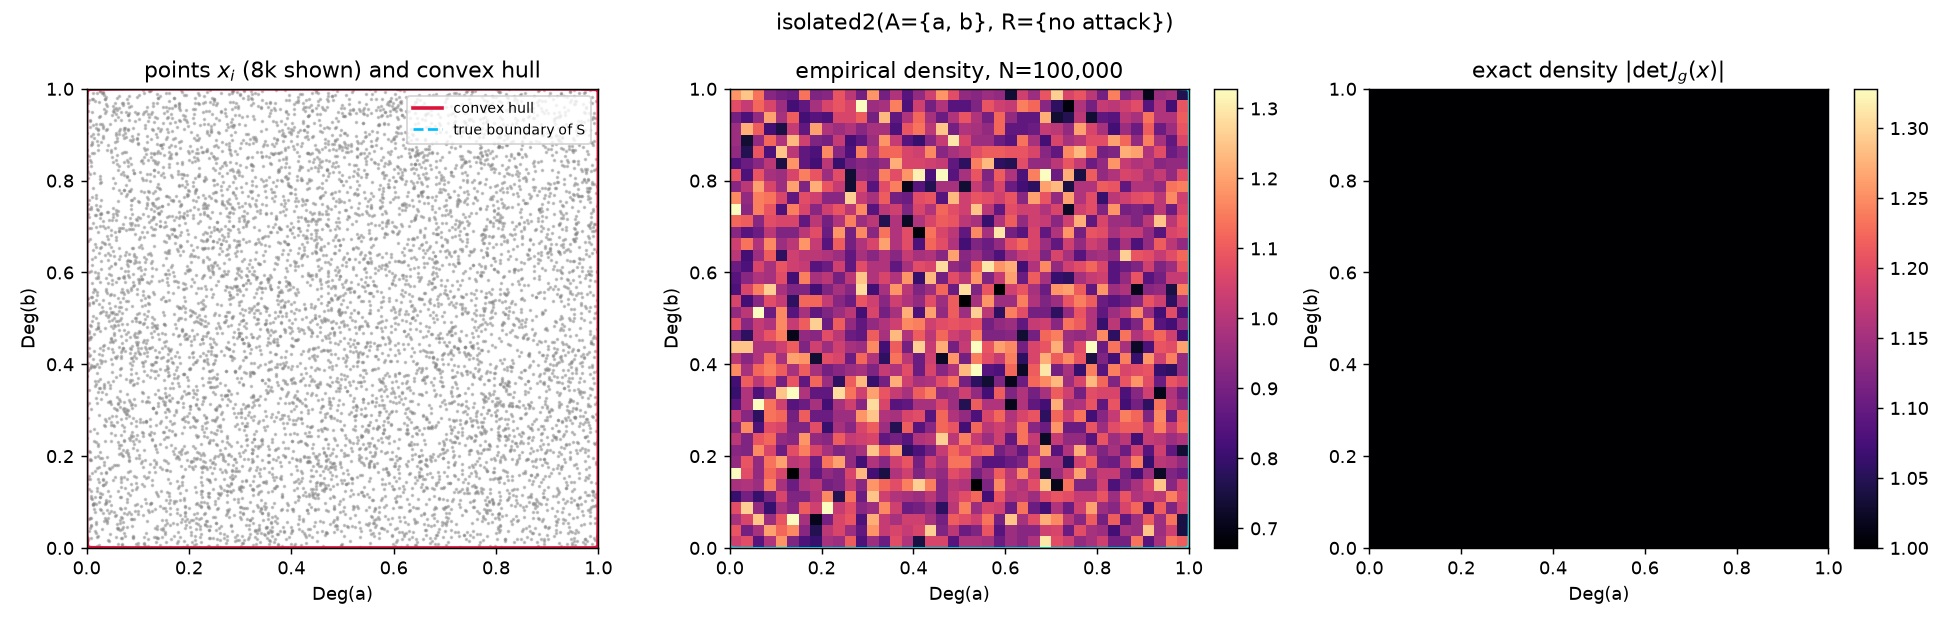
\includegraphics[width=\linewidth]{space_isolated2.png}
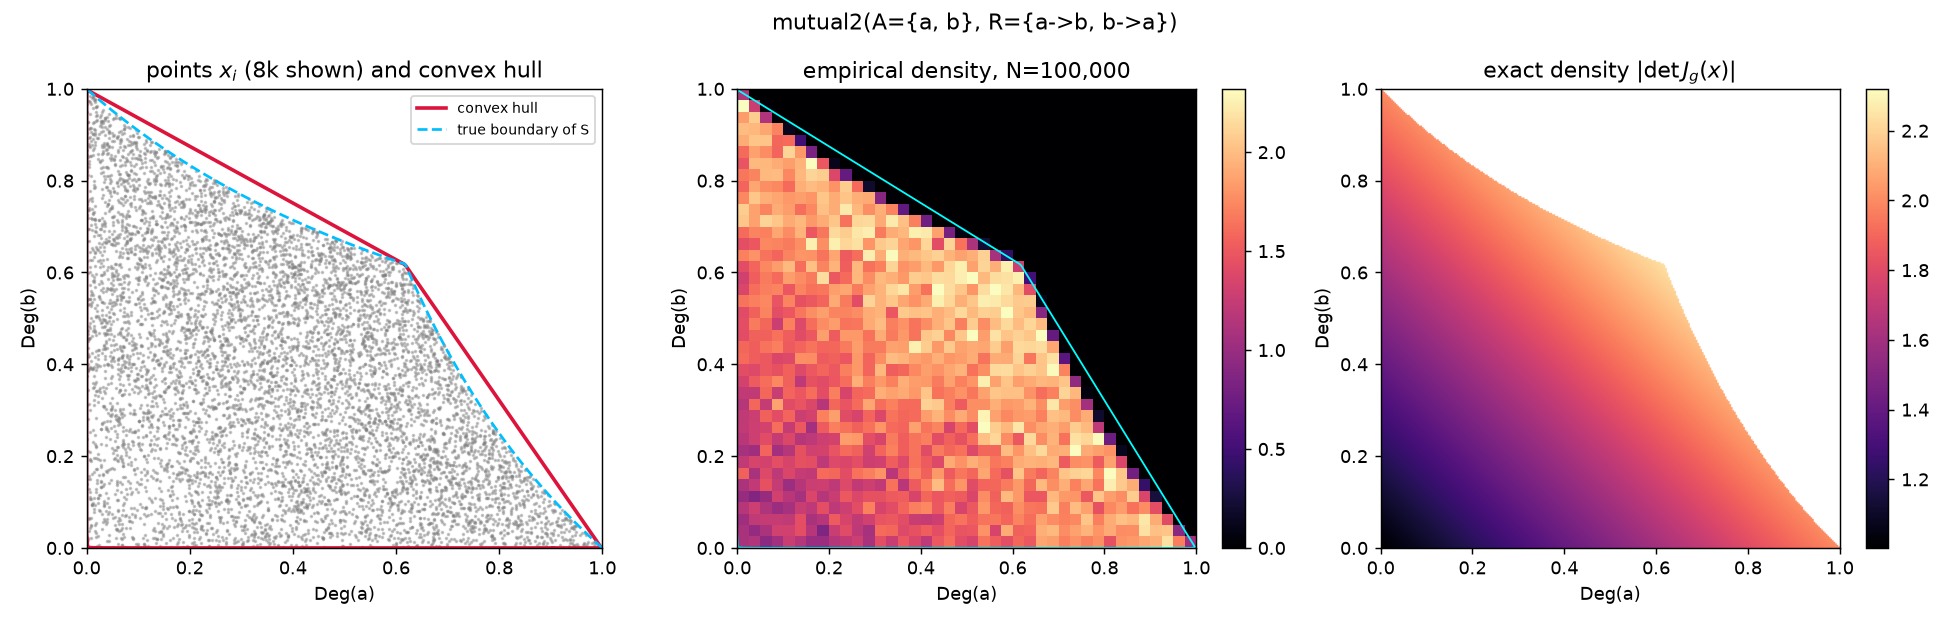
\includegraphics[width=\linewidth]{space_mutual2.png}
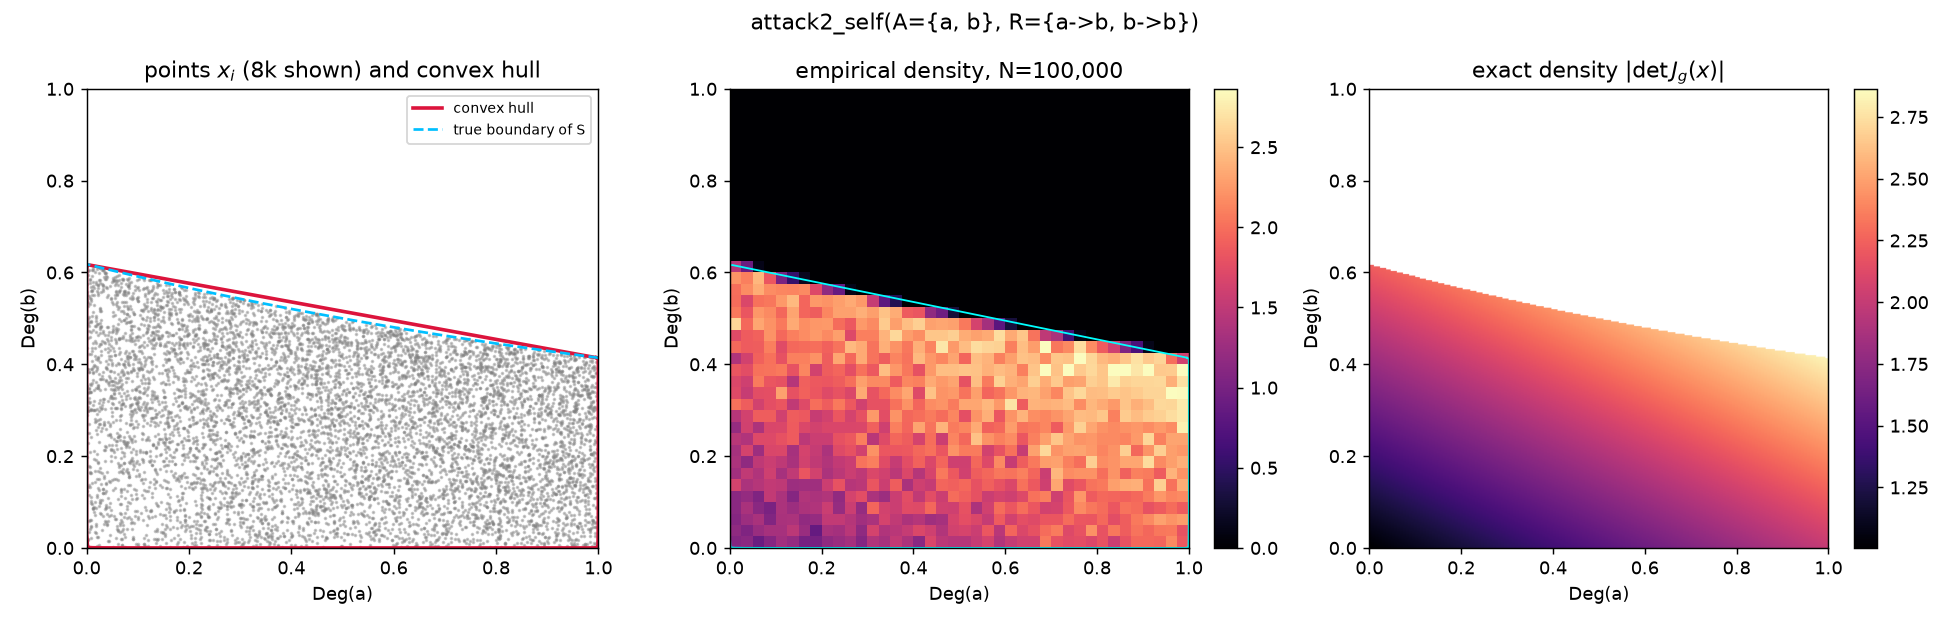
\includegraphics[width=\linewidth]{space_attack2_self.png}
\caption{Sans attaque, attaque mutuelle, et $a\to b$ avec auto-attaque de $b$.}
\end{figure}

\subsection{Frameworks à 3 arguments}
\begin{figure}[H]\centering
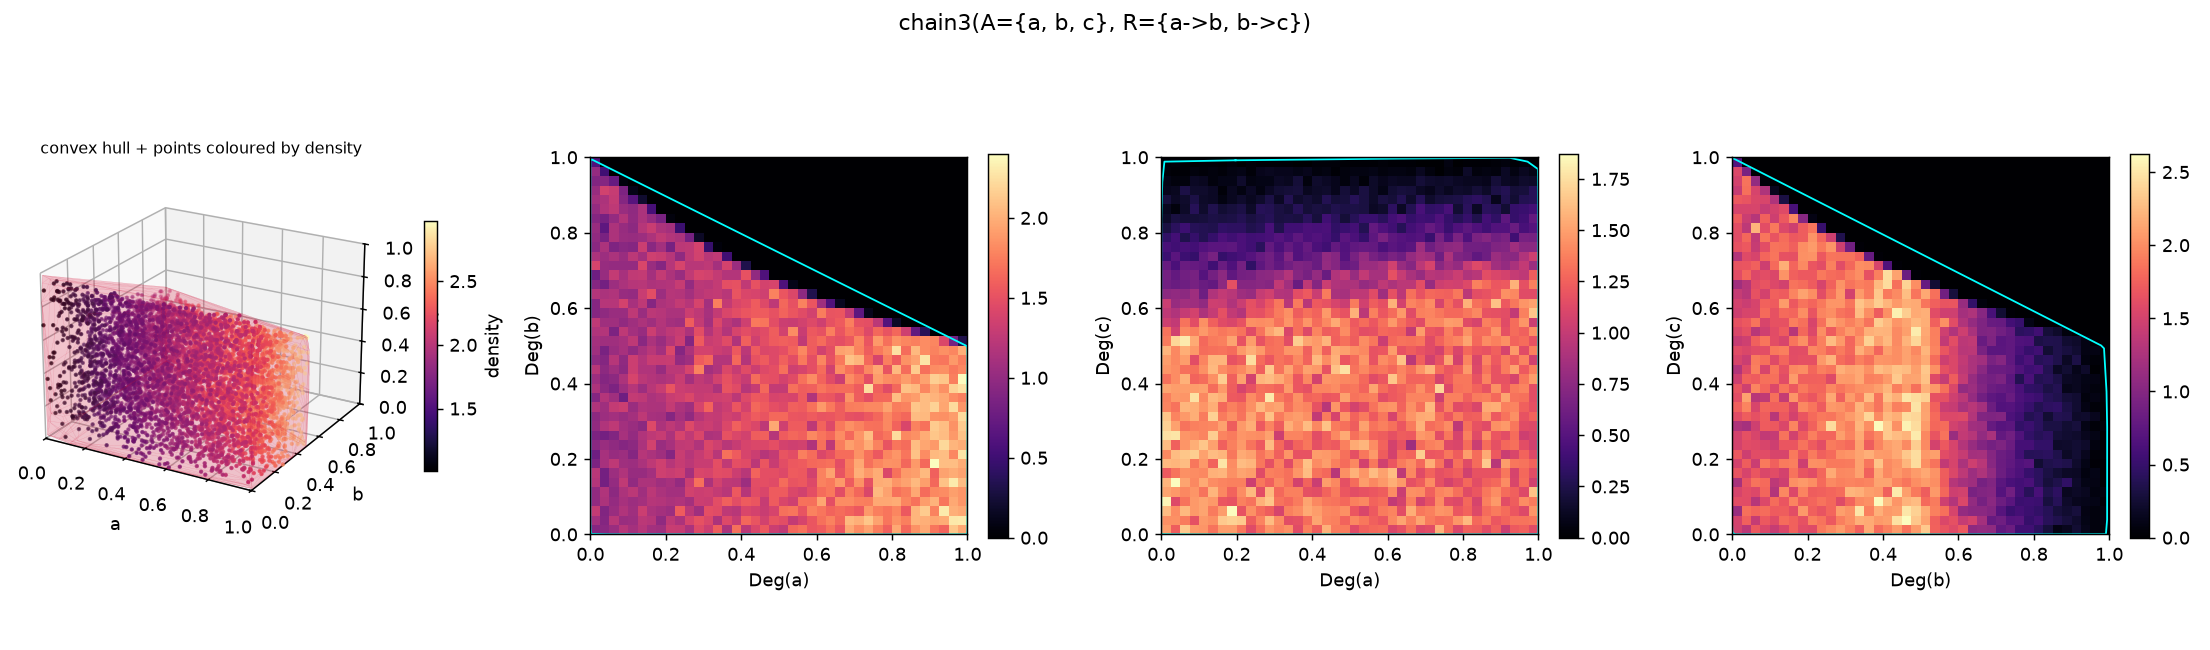
\includegraphics[width=\linewidth]{space_chain3.png}
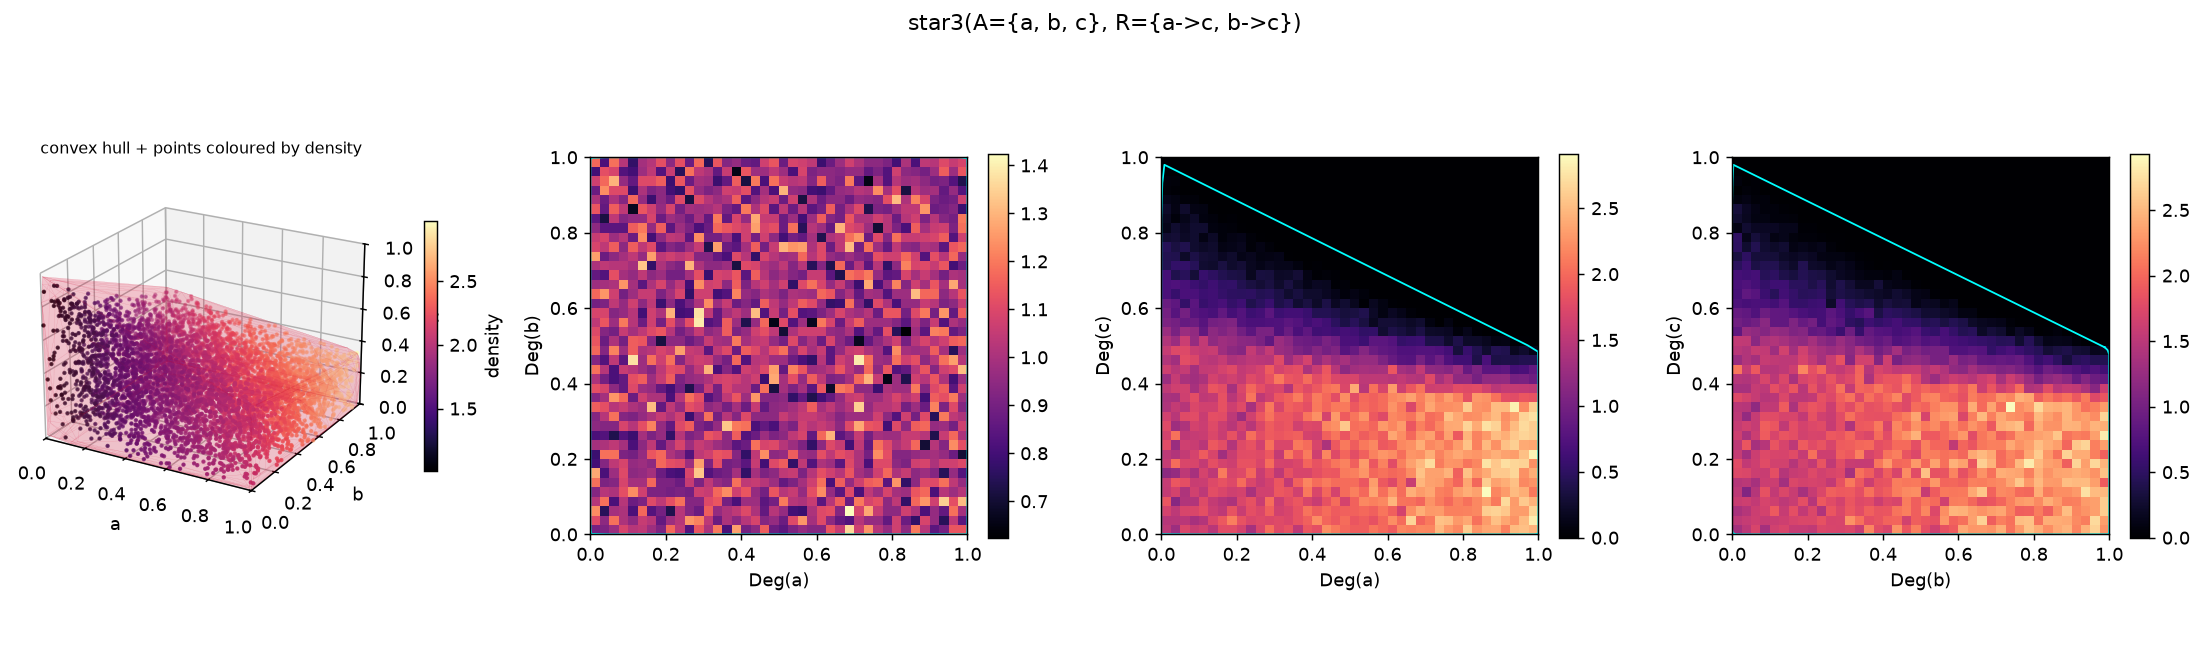
\includegraphics[width=\linewidth]{space_star3.png}
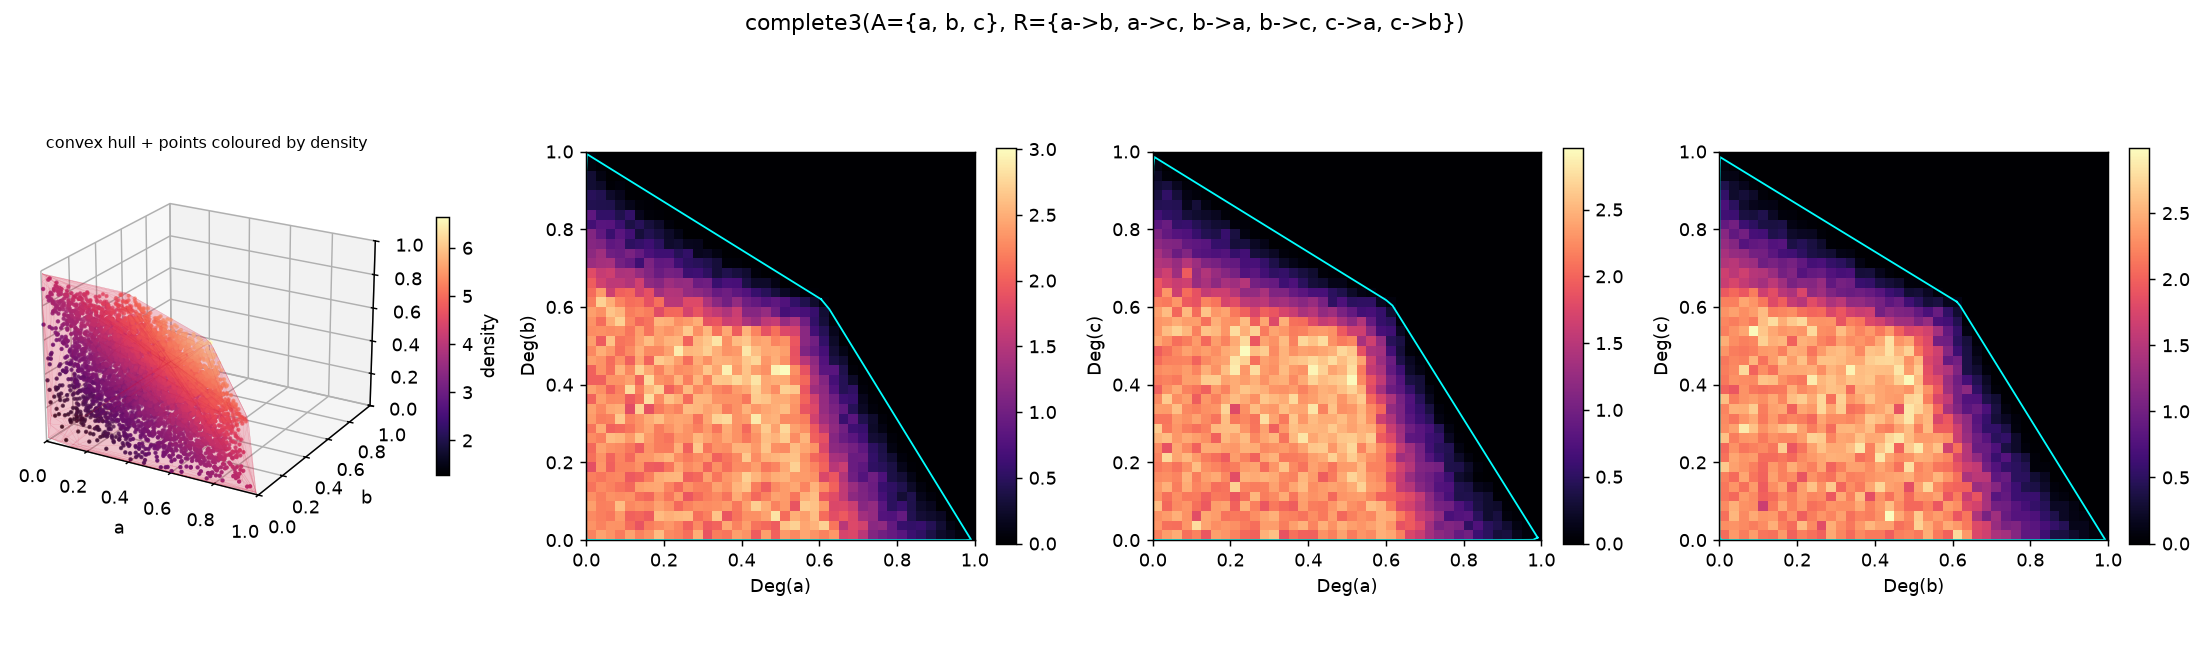
\includegraphics[width=\linewidth]{space_complete3.png}
\caption{Chaîne, étoile et graphe complet à 3 arguments.}
\end{figure}

\subsection{Frameworks à 4 arguments}
\begin{figure}[H]\centering
\begin{subfigure}{0.49\linewidth}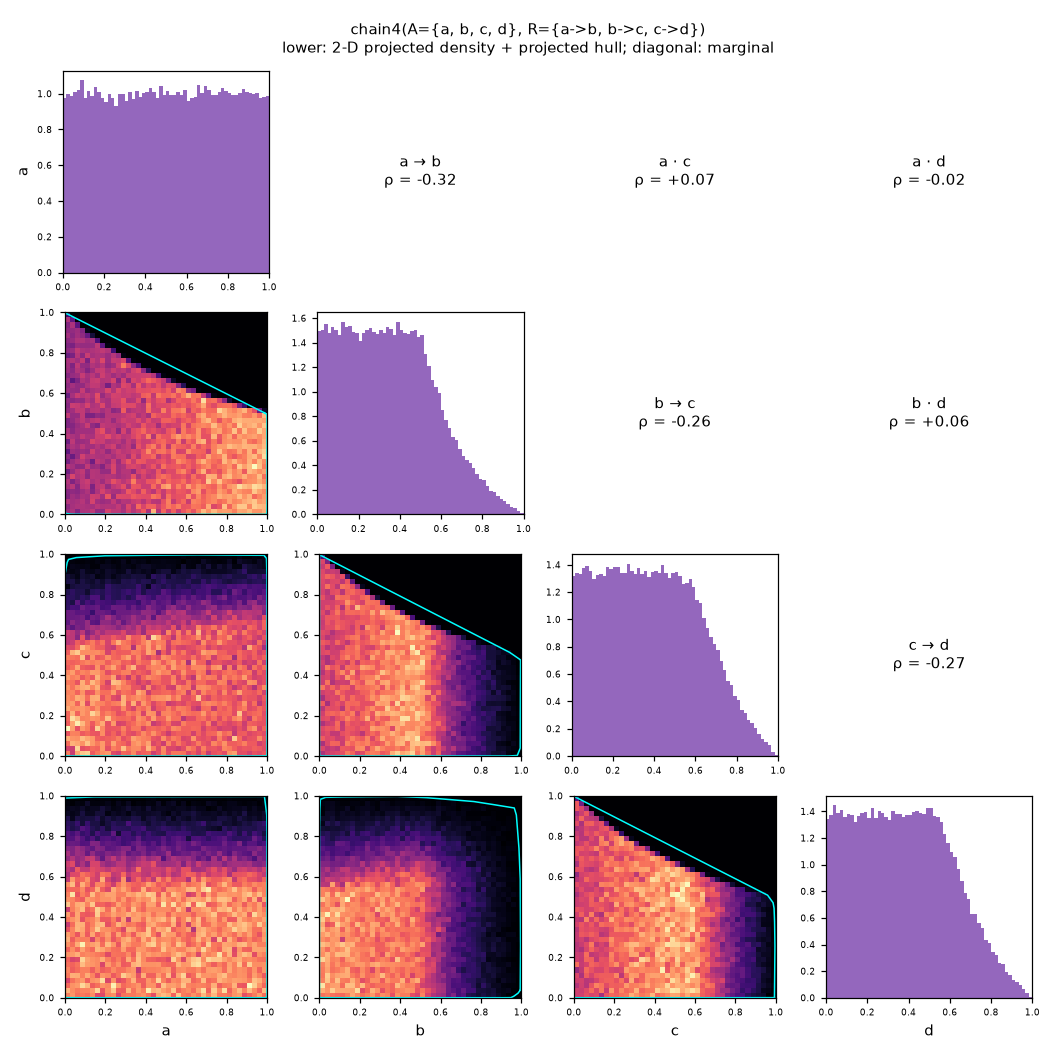
\includegraphics[width=\linewidth]{space_chain4.png}\caption{chaîne}\end{subfigure}
\begin{subfigure}{0.49\linewidth}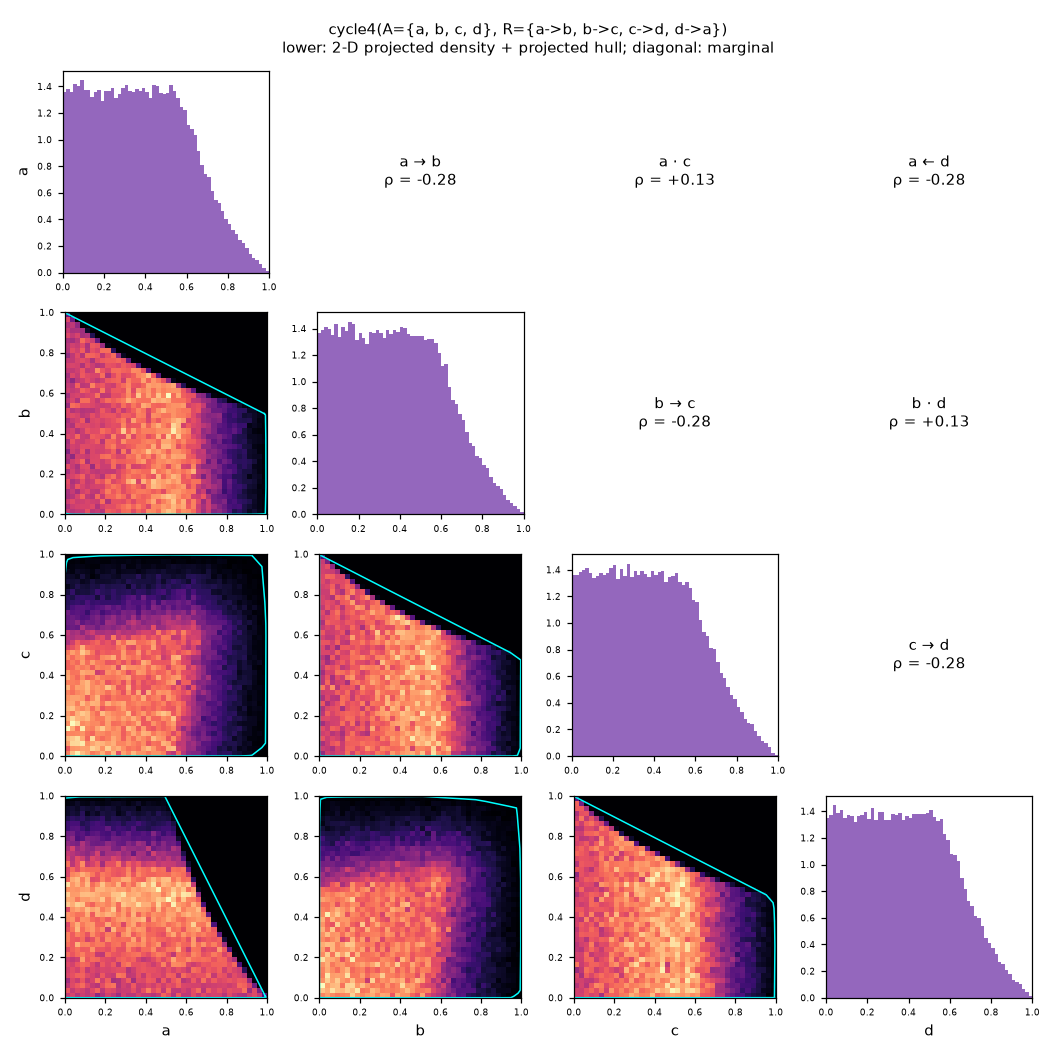
\includegraphics[width=\linewidth]{space_cycle4.png}\caption{cycle}\end{subfigure}
\begin{subfigure}{0.49\linewidth}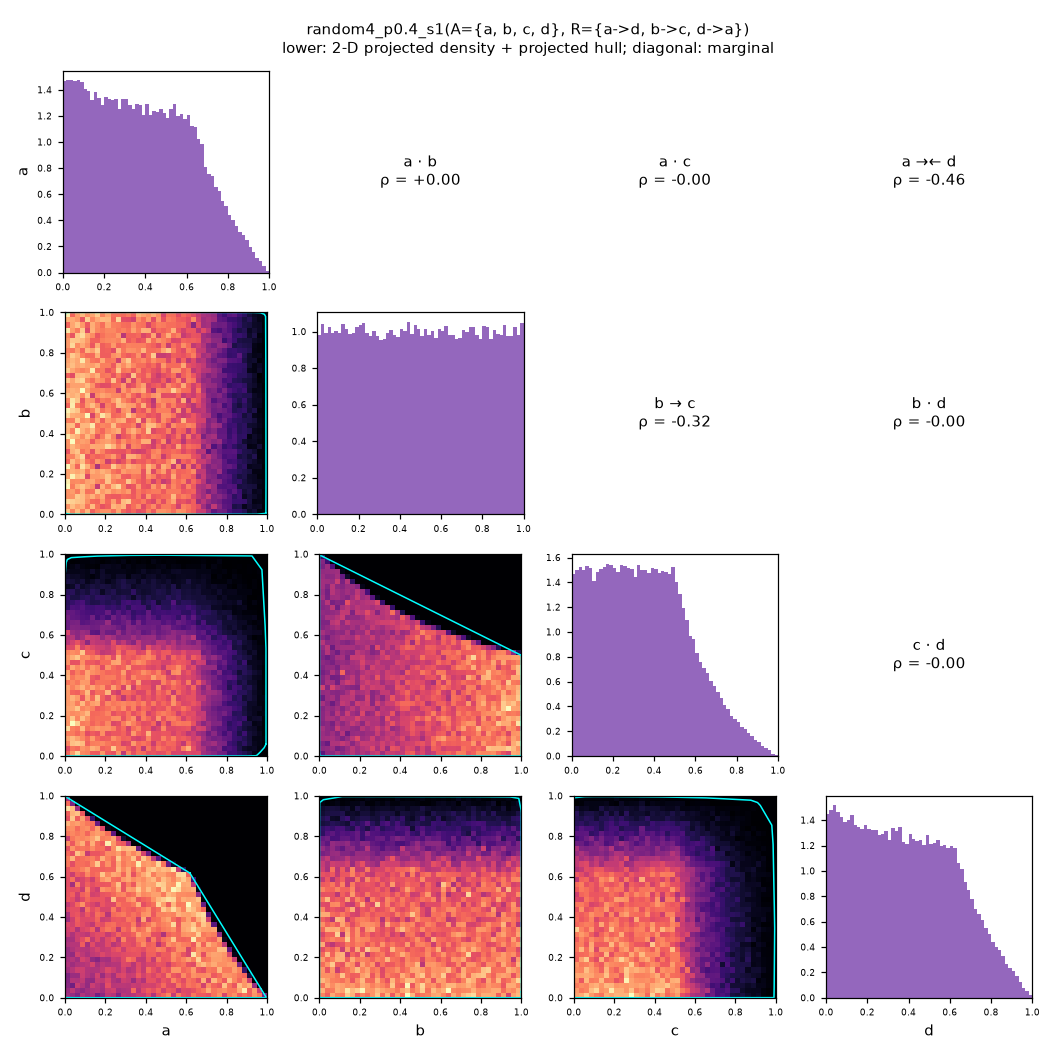
\includegraphics[width=\linewidth]{space_random4_p0.4_s1.png}\caption{aléatoire ($p=0{,}4$)}\end{subfigure}
\caption{Frameworks à 4 arguments (le graphe complet est en figure~\ref{fig:complete4}).}
\end{figure}

\subsection{Frameworks à 5 arguments}
\begin{figure}[H]\centering
\begin{subfigure}{0.49\linewidth}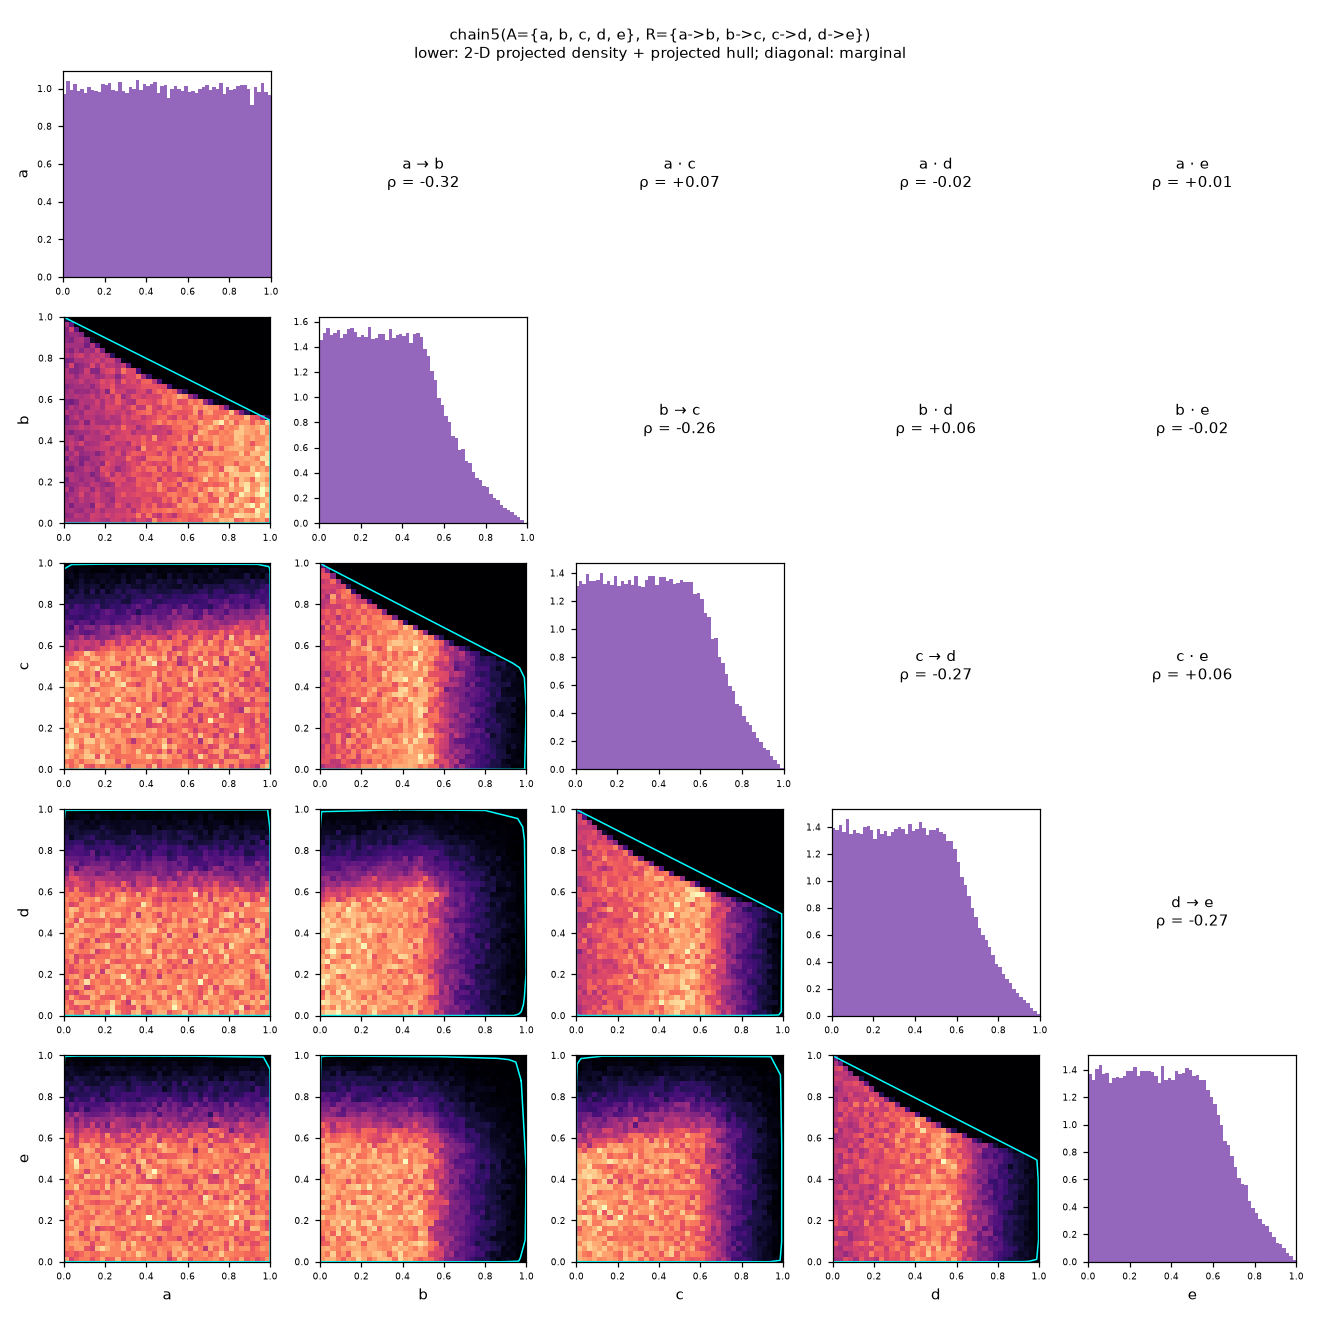
\includegraphics[width=\linewidth]{space_chain5.png}\caption{chaîne}\end{subfigure}
\begin{subfigure}{0.49\linewidth}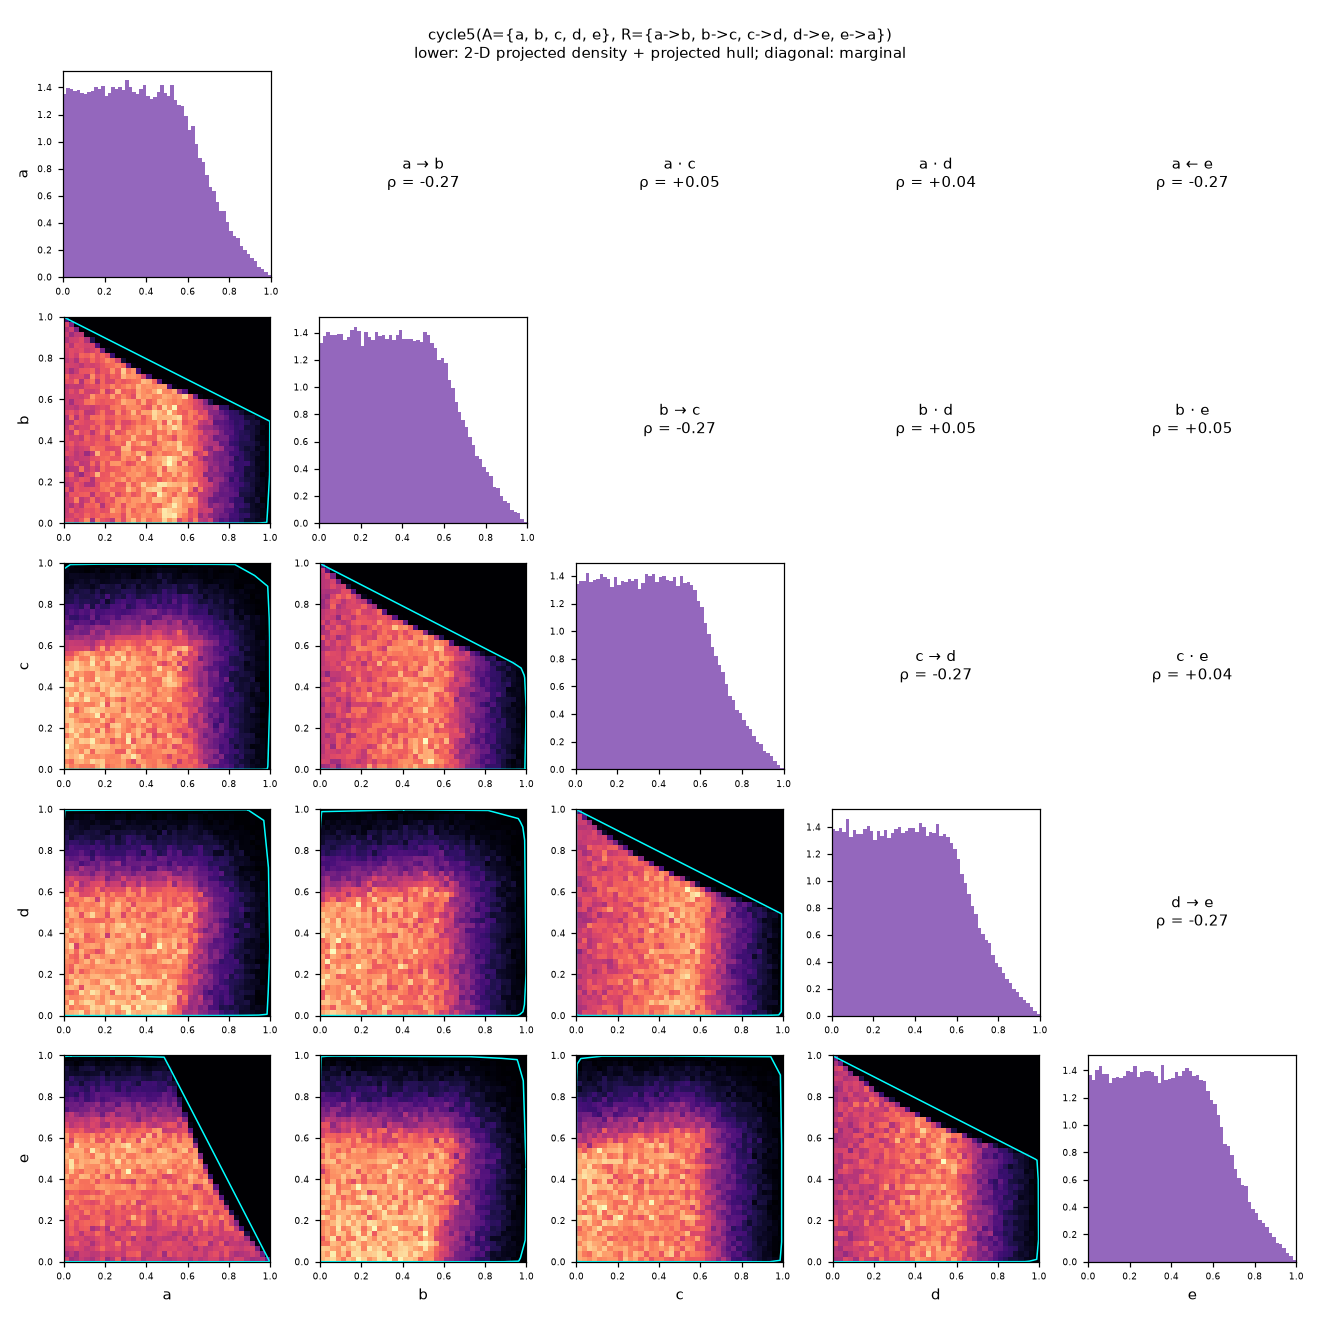
\includegraphics[width=\linewidth]{space_cycle5.png}\caption{cycle}\end{subfigure}
\begin{subfigure}{0.6\linewidth}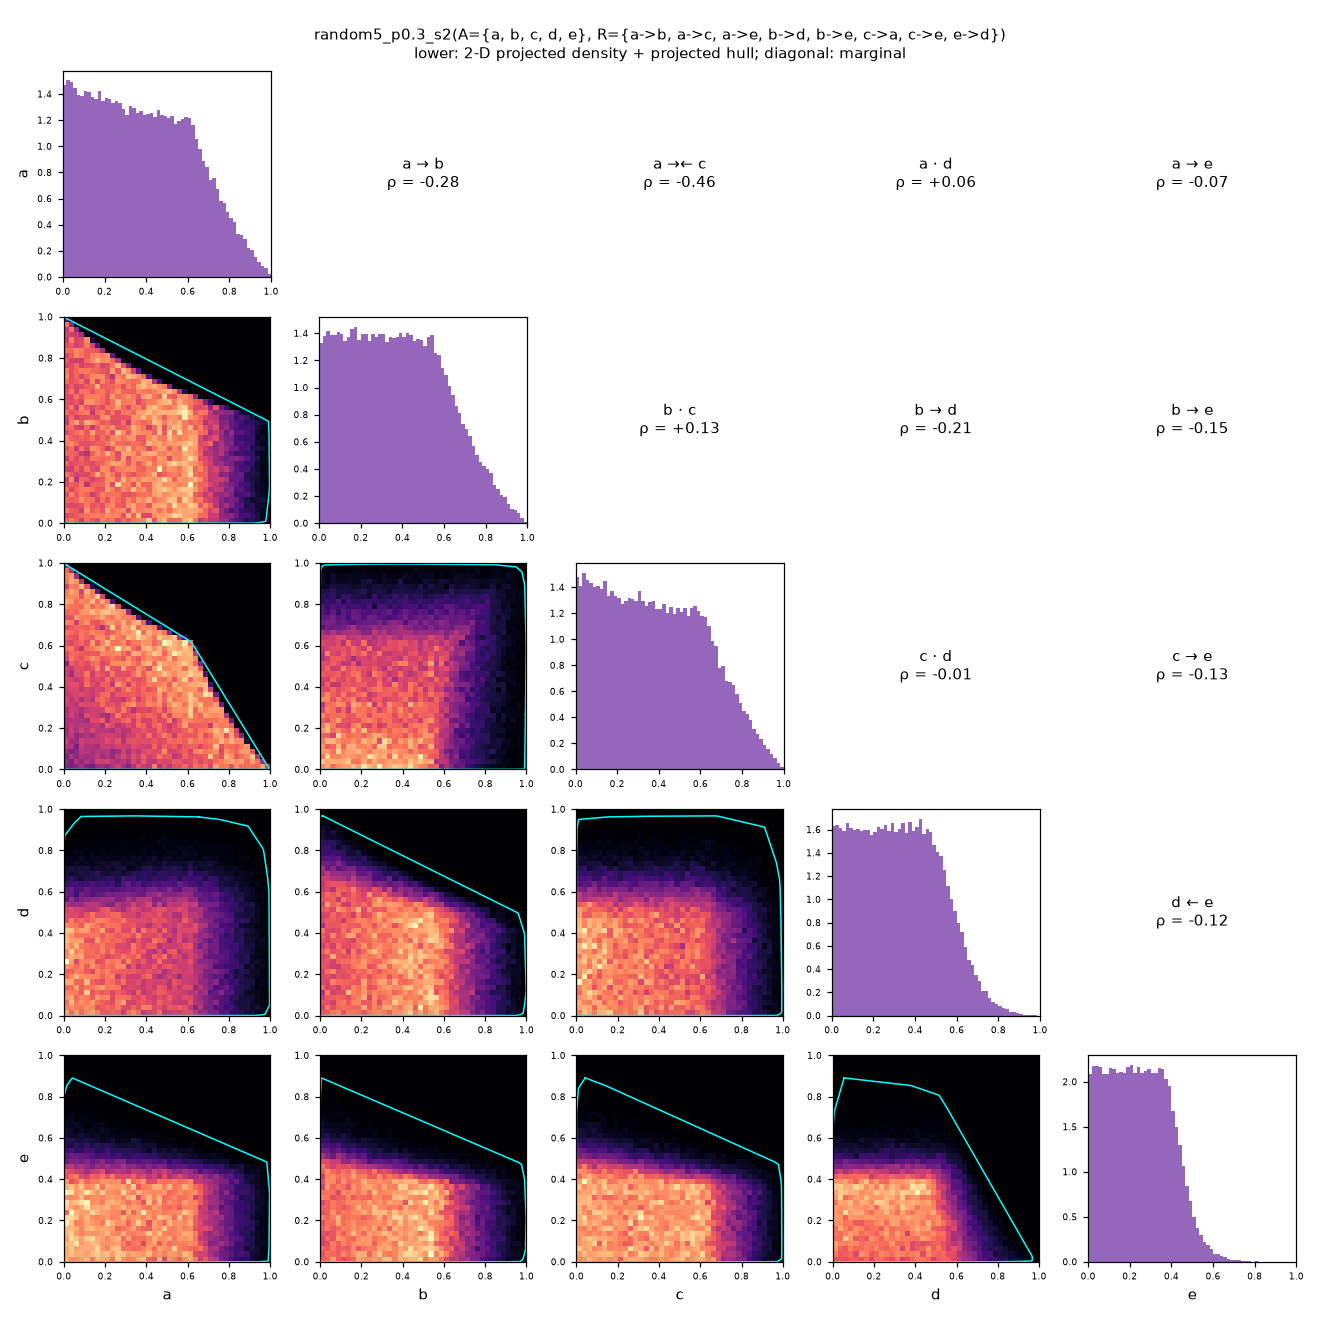
\includegraphics[width=\linewidth]{space_random5_p0.3_s2.png}\caption{aléatoire ($p=0{,}3$)}\end{subfigure}
\caption{Frameworks à 5 arguments.}
\end{figure}

\subsection{Frameworks à 6 arguments}
\begin{figure}[H]\centering
\begin{subfigure}{0.49\linewidth}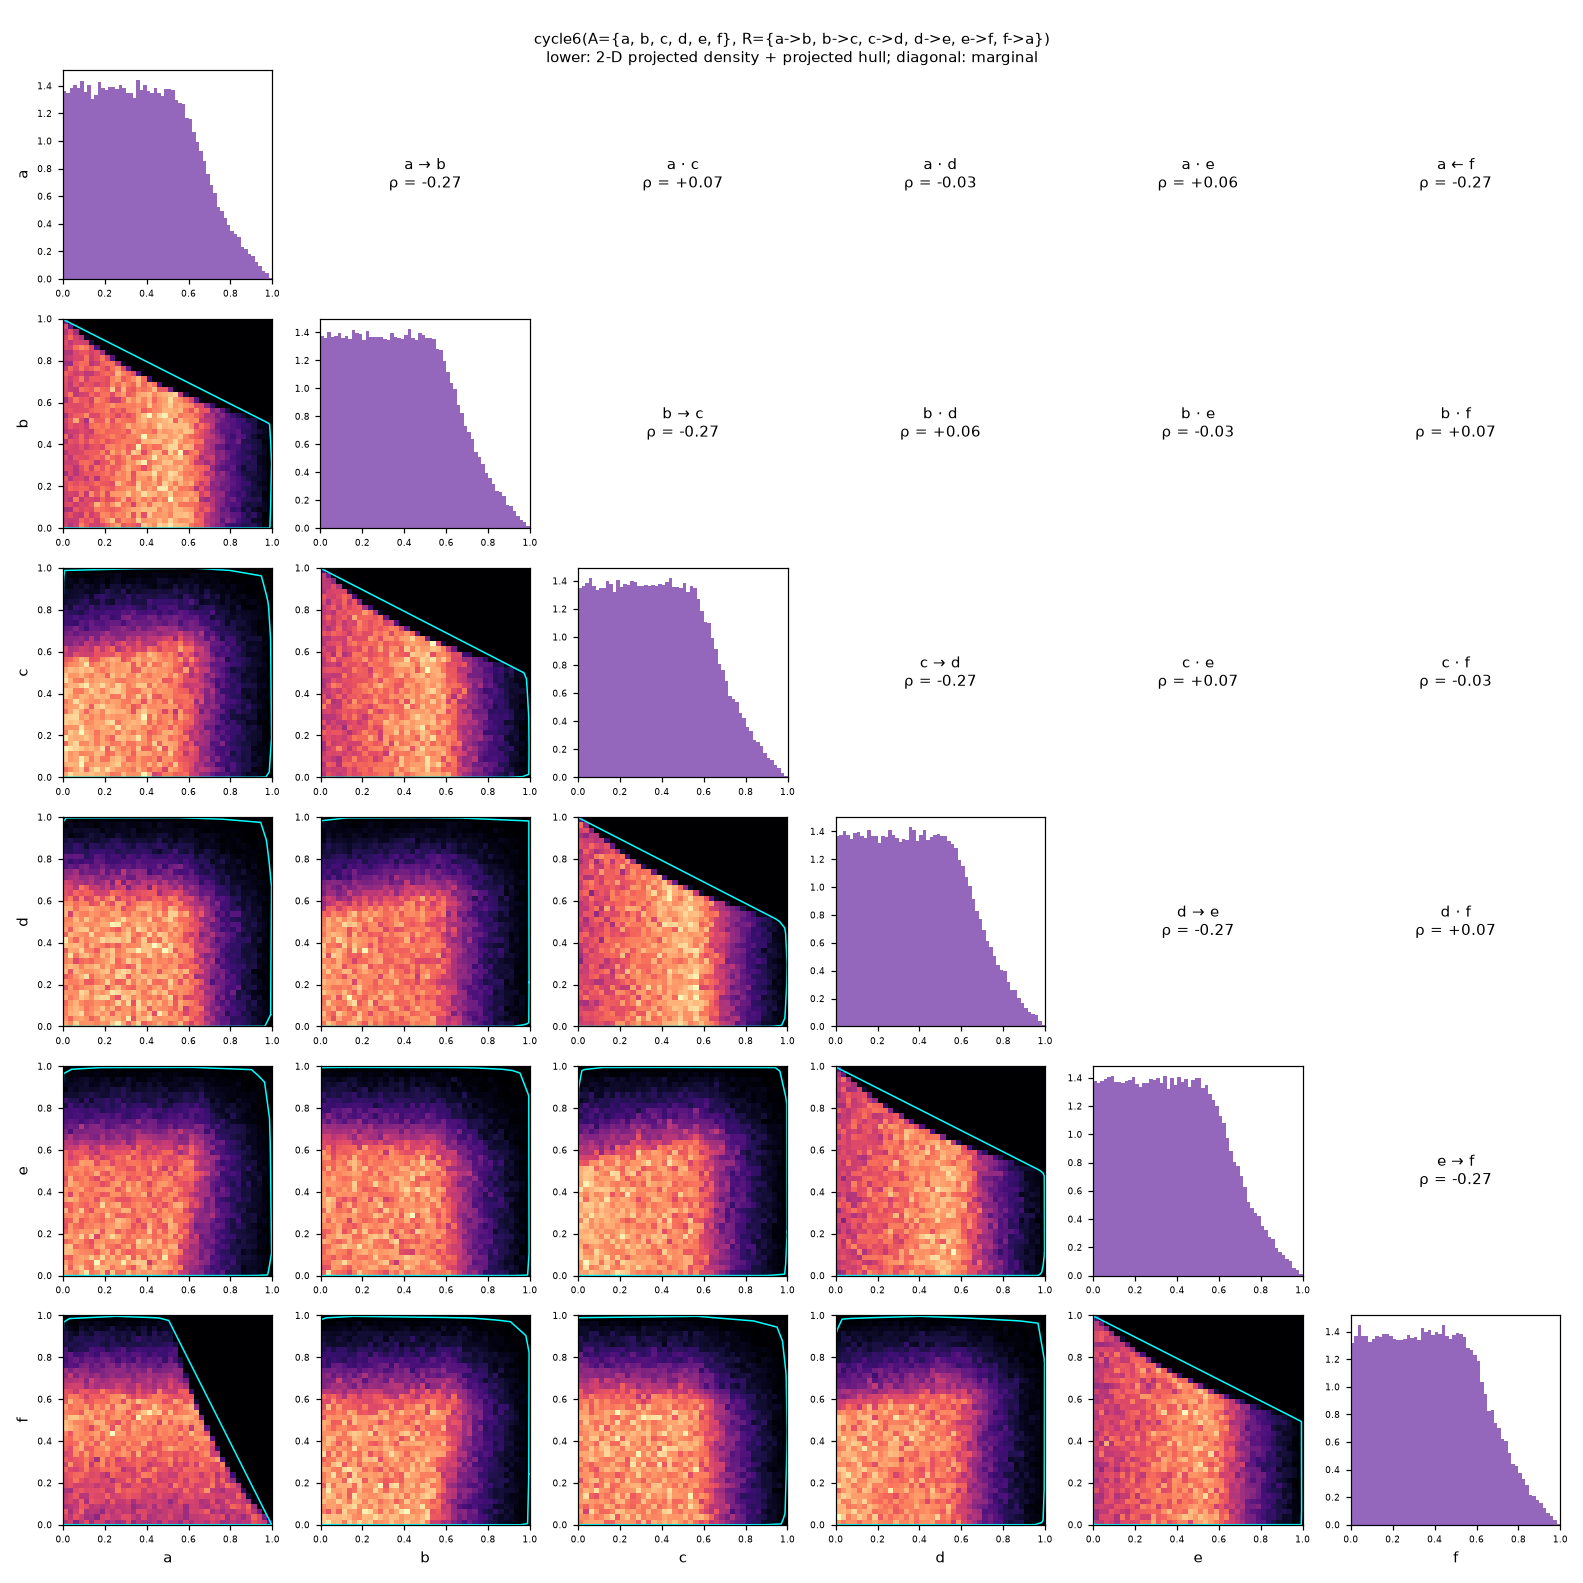
\includegraphics[width=\linewidth]{space_cycle6.png}\caption{cycle}\end{subfigure}
\begin{subfigure}{0.49\linewidth}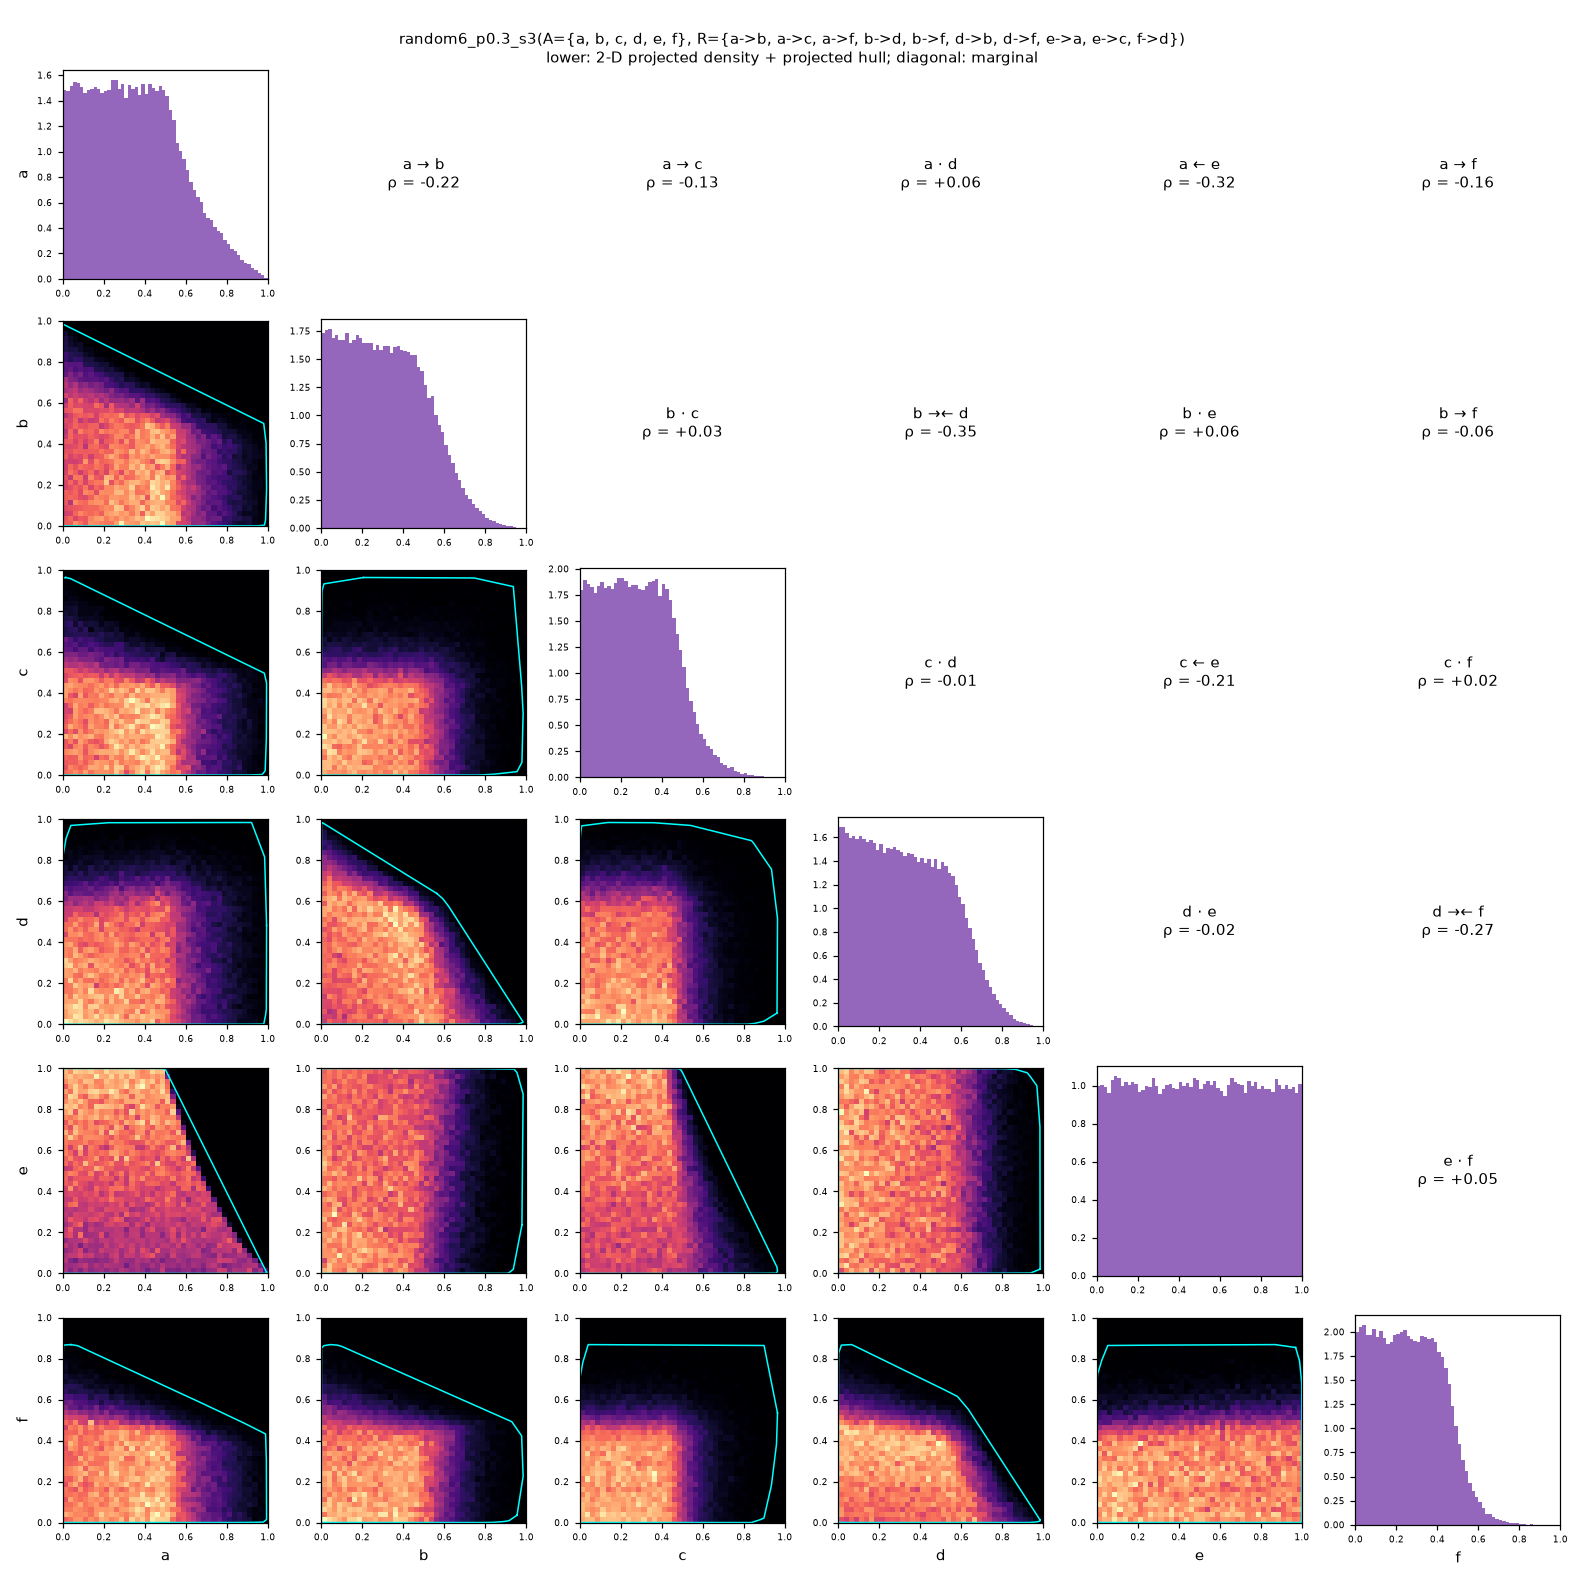
\includegraphics[width=\linewidth]{space_random6_p0.3_s3.png}\caption{aléatoire ($p=0{,}3$)}\end{subfigure}
\caption{Frameworks à 6 arguments.}
\end{figure}

\subsection{Ré-échantillonnage}
\begin{figure}[H]\centering
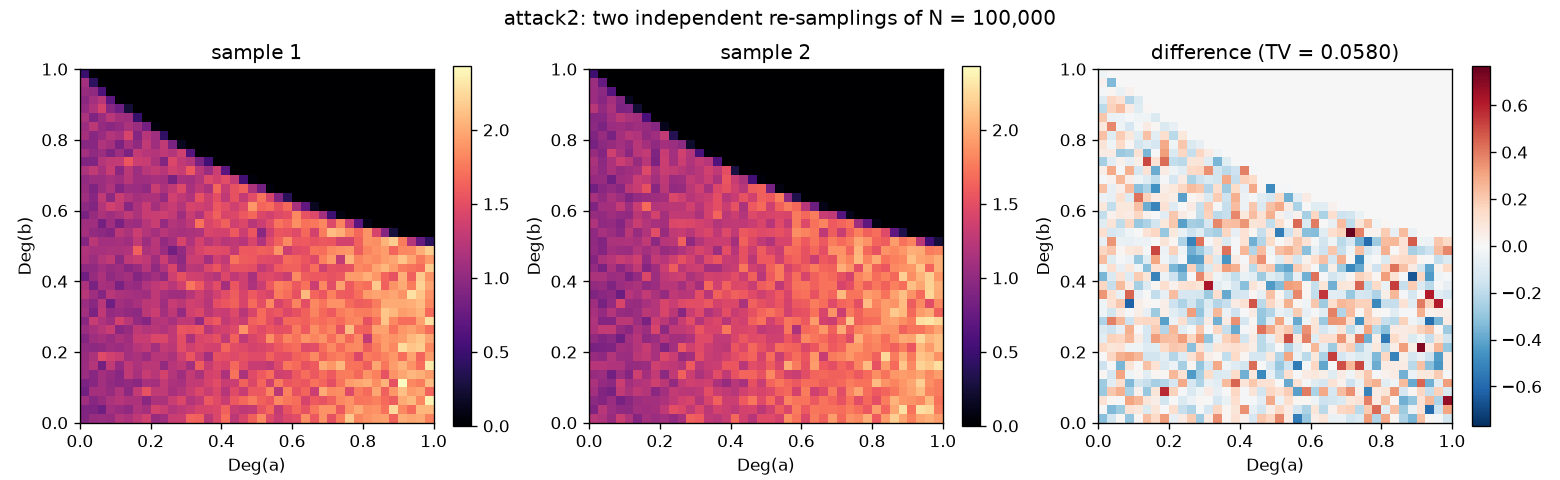
\includegraphics[width=\linewidth]{resampling_attack2.png}
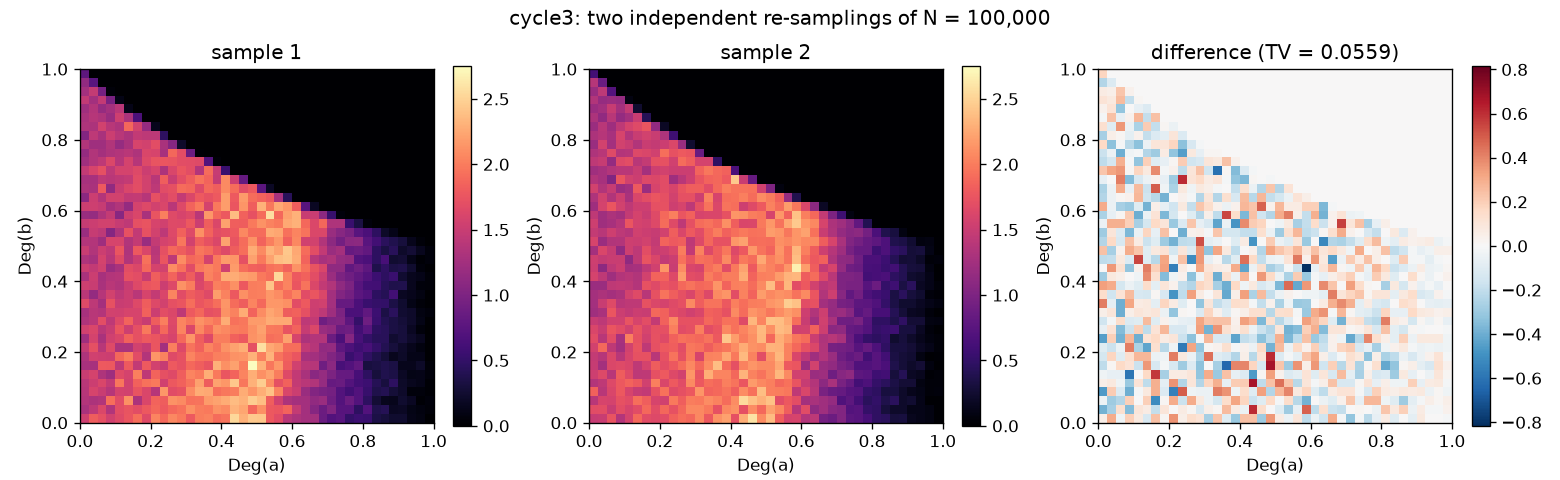
\includegraphics[width=\linewidth]{resampling_cycle3.png}
\caption{Deux ré-échantillonnages indépendants et leur différence, pour $a\to b$ et le cycle à 3.}
\end{figure}

\end{document}
